\documentclass[a4,12pt]{horizon-theme}
\usepackage{enumitem}

\setTitle{Sistema Inteligente para Descoberta em Astronomia}
\setUniversity{Universidade de São Paulo}
\setFaculty{Escola Politécnica}
\setDepartment{Departamento de Eng. da Computação e Sist. Digitais}
\setCoverMainLogo{figures/minerva.pdf}

\setCoverLeftBox{%
  {\Large Especificação Detalhada}\\[2pt]
  {PCS3550 -- Projeto de Formatura I}\\[75pt]
  {\Large Natanael Magalhães Cardoso}\\[10pt]
  {\large \textsc{Orientador:} Prof. Dr. Antonio Mauro Saraiva}
}

\setCompactAuthors{Natanael Magalhães Cardoso\textsuperscript{{\large $\star$}, \faEnvelope[regular]},%
%, Prof. Cláudia Mendes de Oliveira\textsuperscript{$\dagger$}}
{ } Prof. Dr. Antonio Mauro Saraiva\textsuperscript{{\large $\star$}, $\dagger$}}

\setHeaderRight{N. M. Cardoso}
\setHeaderLeft{Escola Politécnica}

\setCompactInfo{\textsuperscript{\large $\star$} {\small Departamento de Engenharia de Computação e Sistemas Digitais, Escola Politécnica, Universidade de São Paulo.}\\[10pt]
\textsuperscript{$\dagger$} {\small Orientador}\\[10pt]
% \textsuperscript{$\dagger$} {\small Departamento de Astronomia, Instituto de Astronimia, Geofísica e Ciências Atmosféricas, Universidade de São Paulo.}\\[10pt]
\textsuperscript{\faEnvelope[regular]} {\small contato@natanael.net}\\[10pt]
{\color{gray}\rule{\linewidth}{0.4pt}}\\[10pt]
{\bf Palavras-chave:} base de conhecimento, visão computacional, vision transformers, aprendizagem profunda, busca por similaridade, astronomia extra-galática, classificação morfológica.}

\setAbstract{A astronomia produz um volume imenso de dados, principalmente na forma de imagens capturadas por telescópios e outros instrumentos. A análise dessas imagens é vital para entender o universo, descobrir novos objetos celestes e fenômenos astronômicos. Nesse sentido, este projeto aborda a aplicação de métodos de aprendizagem profunda e visão computacional na astronomia, com ênfase na análise de imagens astronômicas. O objetivo é criar um sistema inteligente que facilite descobertas astronômicas composto por um modelo de aprendizagem profunda capaz de extrair representações visuais de alta qualidade, uma base de dados para armazenar as representações obtidas e uma aplicação web para possibilidar uma exploração intuitiva de uma base dados astronômica.}

% \setAbstract{Este trabalho apresenta uma abordagem inovadora para criar uma base de conhecimento para busca por similaridade visual, utilizando embeddings gerados pelo modelo MaxViT, um transformer de visão, em conjunto com o algoritmo HNSW para fornecer uma interface web eficaz e acessível. O MaxViT, uma variação do Transformer, demonstrou excelentes resultados na extração de representações visuais de alta qualidade, enquanto o HNSW possibilita uma busca rápida e escalável dentro do espaço de embeddings. Essa combinação oferece uma base de conhecimento robusta e eficiente, capacitando os usuários a explorarem vastos conjuntos de dados visuais de maneira intuitiva e precisa. A interface web desenvolvida oferece uma experiência de busca visualmente rica, permitindo aos usuários carregar uma imagem de consulta ou fornecer uma descrição textual para recuperar imagens semelhantes a partir do banco de dados.} %Com recursos como visualização de resultados, filtragem por categoria e personalização de preferências de busca, a interface torna a busca por imagens uma experiência altamente interativa e envolvente %Além disso, a acessibilidade universal da plataforma, que pode ser acessada de qualquer dispositivo conectado à Internet, amplia seu alcance e utilidade, proporcionando uma solução flexível e conveniente para a exploração de conteúdo visual.}

% Contudo, uma classificação morfológica feita através de inspeção visual está sujeita a um viés causado pela subjetividade da observação humana. Neste trabalho,  propomos um modelo de \emph{Deep Learning} treinado a partir de classificações visuais do GalaxyZoo e imagens do Legacy Survey. O objetivo é obter um modelo de \emph{Deep Learning} que seja capaz de classificar galáxias mergers com magnitude $r < 17.5$}



\definecolor{myred}{rgb}{0.99, 0.14, 0.12}
\newcommand{\natanael}[3]{{\fcolorbox{myred}{myred}{\color{white}Item #1:}} {\color{myred}\sout{#2}} {\color{myred} #3}}


\newcolumntype{Y}{>{\raggedleft\arraybackslash}X}
% \rowcolors{2}{blue!5!white}{blue!15!white}
\newtcolorbox[blend into=tables]{htable}[4]{%
    enhanced,
    fonttitle=\bfseries,
    colback=white,
    colframe=secondaryColor!90!white,
    colbacktitle=secondaryColor!90!white,
    coltitle=white,
    center title,
    halign title=center,
    toptitle=40pt,
    bottomtitle=40pt,
    boxrule=.8pt,
    float=!htb,
    title=\strut {#2},
    tabularx*={\arrayrulewidth0.4mm\renewcommand{\arraystretch}{1.5}}{#1},
    before upper app={#3\\\hline\hline},
    label={#4},
}


\usepackage{translator}
\usepackage{pgfgantt}
\AtBeginEnvironment{ganttchart}{\deftranslation[to=Brazilian]{May}{Mai}}
\definecolor{barblue}{RGB}{153,204,254}
\definecolor{groupblue}{RGB}{51,102,254}


\addbibresource{refs.bib}
\begin{document}
\horizonCover

\horizonTitle

\horizonAbstract

\newpage

\tableofcontents

\newpage

\onehalfspacing
\section{Introdução}
A astronomia é uma das ciências que mais gera dados, especialmente na forma de imagens obtidas através de telescópios terrestres e espaciais e instrumentos acoplados a estes \citep{astronomy_bigdata}. A análise dessas imagens é crucial para a compreensão de como funciona o universo e responder perguntas tão fundamentais quanto de onde viemos e para onde vamos. A análise de imagens astronômicas também é importante para a descoberta de novos objetos celestes de tipos já conhecidos e até mesmo de novos fenômenos astronômicos, nunca antes vistos, trazendo novos desafios e novas perguntas a serem respondidas. Em 10 de abril de 2019, por exemplo, foi publicado o primeiro imageamento de um buraco negro, no centro da galáxia de M87, com imagens maravilhosas, como da Fig. \ref{fig:m87_blackhole}, que correram os jornais do mundo inteiro \citep{M87_blackhole}.

\begin{figure}[!ht]
  \centering
  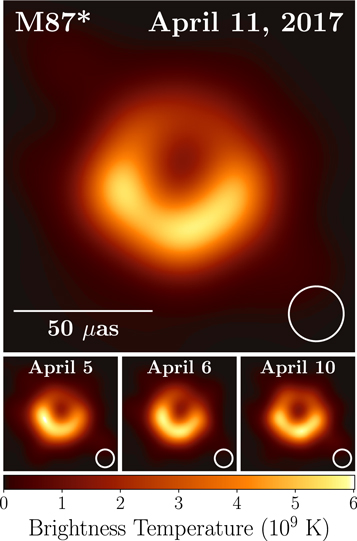
\includegraphics[width=0.45\textwidth]{figures/M87_blackhole.png}
  \caption[Primeiro imageamento de um buraco negro.]{Primeiro imageamento de um buraco negro. Fonte: \emph{The Event Horizon Telescope Collaboration et al., 2019}.}
  \label{fig:m87_blackhole}
\end{figure}

Outro bom exemplo foi o que aconteceu em agosto de 2017, quando houve a primeira detecção em imagem óptica de uma onda gravitacional vinda da fusão de duas estrelas de nêutrons. Essas são estrelas muito densas, já colapsadas, em um sistema binário, que quando se fundem provocam uma explosão parecida mas menos intensa que de uma supernova, formando o que é chamado de uma kilonova. O mundo inteiro se empolgou com tal fenômeno, pois se sabia que o ocorrido seria visto em alguma imagem do céu naquela noite, mas não se sabia exatamente onde (a área de procura no céu onde poderia acontecer era enorme). Finalmente a contrapartida óptica da onda gravitacional foi encontrada, também por brasileiros \citep{estrela_neutrons}, e foi seguida por quase uma centena de telescópios no mundo inteiro por várias noites e desde então a comunidade astronômica procura por outros eventos do mesmo tipo, vasculhando imagens obtidas todas as noites\footnote{\url{https://www.gov.br/observatorio/pt-br/assuntos/noticias/imagens-fusao-estrelas-neutrons}}.

O volume crescente de dados astronômicos, à medida que as pesquisas continuam, torna a tarefa de localizar e analisar imagens específicas extremamente desafiadora para os astrônomos \citep{astronomy_bigdata_challenges}. Tradicionalmente, a busca por imagens astronômicas é realizada através de metadados previamente extraídos de imagens processadas, como a localização no céu (latitude e longitude), propriedades físicas (como o brilho e o diâmetro) e, até mesmo, anotações manuais. Todavia, esse método é limitado e não explora plenamente a riqueza visual contida nas imagens, além de não escalar bem com a quantidade massiva de dados gerada na era dos grandes levantamentos astronômicos, que são telescópios destinados à observação contínua e geração de dados em larga escala.

A cada década se constroem telescópios cada vez maiores, como por exemplo o \emph{Giant Magellan Telescope} (GMT, \cite{gmt}) e o \emph{Extremely Large Telescope} (ELT, \cite{elt}) ou se constroem telescópios com cada vez mais capacidade de se obter dados, como o \emph{Large Synoptic Survey Telescope} (LSST) ou \emph{Vera Rubin Observatory} \citep{lsst}. Esse último, o \emph{LSST/Vera Rubin} é uma das motivações deste projeto. Trata-se de um projeto que irá começar a tomar dados no próximo ano e haverá um volume de petabytes de dados a cada ano provenientes deste telescópio, imagens que têm que ser exploradas de forma eficiente. Este trabalho é um esforço de fazer ferramentas para explorar tais dados no futuro. Neste trabalho, serão usadas as imagens do levantamento \emph{Legacy Survey} \citep{legacy} obtidas pelo instrumento \emph{Dark Energy Camera}, que têm uma estrutura muito parecida com as imagens que serão obtidas pelo projeto futuro \emph{LSST/Vera Rubin}.

Através de discussões com astrônomos profissionais e professores do IAG que estão acostumados a lidar com imagens astronômicas e estão preocupados com a enorme quantidade de dados que o LSST trará, quando começar a funcionar, definimos a direção deste trabalho para que seja útil também para a comunidade astronômica. Nós identificamos que o importante no momento para a exploração das imagens em grandes levantamentos como os do \emph{Dark Energy Survey} ou LSST, é desenvolver uma forma automática de realizar buscas por similaridade visual em grandes conjuntos de dados astronômicos. Isso é possível devido à capacidade de extração de representações visuais pelos modelos atuais de visão computacional \citep{cnn_representations}.

Nas últimas décadas, muitas das classificações de galáxias e objetos raros em imagens foram feitas por inspecção do olho humano através do \emph{Galaxy Zoo} \citep{galaxyzoo}, um projeto de ciência cidadã \citep{cs-bonney, cs-naturalscience} que inseriu pela primeira vez na área a colaboração voluntária de membros da sociedade no processo de construção do conhecimento científico em astronomia. Ao decorrer de várias campanhas, o \emph{Galaxy Zoo} coletou milhões de classificações visuais humanas provenientes dos voluntários e que estão disponíveis para uso na ciência.




\section{Metodologia}
\label{sec:metodologia}
O desenvolvimento do sistema inteligente para buscas em astronomia conta com apoio da Profa. Dra. Cláudia Mendes de Oliveira do Grupo de Astronomia Extragalática do Departamento de Astronomia do Instituto de Astronomia, Geofísica e Ciências Atmosféricas (IAG) da Universidade de São Paulo (USP) e será realizado em etapas estruturadas e modulares.


As subseções a seguir, que detalham a metodologia proposta para o desenvolvimento deste trabalho, englobam desde a revisão literária (Seção \ref{sec:revisao}), passando por todas etapas técnicas de implementação  (Seções \ref{sec:preparacao}, \ref{sec:modelo}, \ref{sec:db}, \ref{sec:webapp}), até a comparação dos resultados obtidos com outros trabalhos na literatura (Seção \ref{sec:comparacao}).



\subsection{Revisão Bibliográfica}
\label{sec:revisao}
A revisão bibliográfica para este projeto multidisciplinar será realizada de maneira abrangente e sistemática, envolvendo as áreas de aprendizagem profunda, visão computacional e astronomia, como descrito nas subseções a seguir.

\subsubsection{Definição dos Objetivos e das Fontes de Informação}
É necessário estabelecer os objetivos específicos da revisão, identificando as principais áreas de estudo a serem abordadas, incluindo métodos de aprendizado profundo, técnicas de visão computacional aplicadas à análise de imagens astronômicas e sistemas de busca por similaridade visual.

Para tanto, é importante utilizar diversas bases de dados acadêmicas relevantes para as áreas de computação e astronomia, como o Portal Periódicos (\url{www.periodicos.capes.gov.br}), o \emph{Google Scholar} (\url{https://scholar.google.com}) e o \emph{Astrophysics Data System} (ADS) (\url{www.adsabs.harvard.edu}), além de conferências relevantes nas áreas de inteligência artificial, processamento de imagens e astronomia, como a \emph{International Conference on Machine Learning} (ICML), a \emph{International Conference on Computer Vision} (ICCV) e a \emph{Astronomical Data Analysis Software and Systems Conference} (ADASS).

Além disso, repositórios de \emph{pré-prints}, como o arXiv (\url{www.arxiv.org}), mantido pela \emph{Cornell University}, ou o TechRxiv (\url{www.techrxiv.org}), mantido pelo \emph{Institute of Electrical and Electronics Engineers} (IEEE), são especialmente úteis por ser um repositório de artigos ainda publicados, sendo úteis para mater a atulização dos estudos emergentes.

A pesquisa em repositórios de produção científica das diferentes áreas -- astronomia, visão computacional e aprendizagem profunda -- abrirá novos horizontes de conhecimento, pois a integração de conhecimentos multidisciplinares promoverá avanços significativos, não apenas no contexto do projeto, mas também contribuindo para o progresso das áreas de estudo envolvidas.



\subsubsection{Seleção e Análise dos Estudos}
Para selecionar estudos relevantes para este trabalho dentre o vasto repertório científico disponível, é importante aplicar critérios de inclusão e exclusão para selecionar artigos, livros, teses e outros materiais relevantes. O objetivo é priorizar estudos que apresentem metodologias avançadas e resultados comprovados, bem como revisões de literatura anteriores que ofereçam uma visão geral das tendências e lacunas nas áreas envolvidas.

Juntamente com seleção, é importante realizar uma leitura crítica dos materiais selecionados, avaliando a qualidade metodológica, a relevância dos resultados e a aplicabilidade das técnicas descritas. Além disso, é necessário identificar as abordagens mais promissoras e as limitações dos estudos existentes, com foco na integração entre aprendizagem profunda, visão computacional e astronomia.


\subsubsection{Síntese e Documentação dos Estudos}
Para que os estudos relevantes selecionados sejam facilmente encontrados em uma consulta posterior, é importante organizar as informações coletadas em categorias temáticas, como técnicas de extração de características visuais em imagens astronômicas, arquiteturas de redes neurais profundas específicas para análise de imagens, algoritmos de busca por similaridade visual, e aplicações práticas na astronomia. Elaborar uma síntese que destaque as principais contribuições, tendências emergentes e áreas de pesquisa futura.

% A documentação dos estudos poderá ser feita compilando os resultados da revisão bibliográfica em um documento estruturado, incluindo resumos dos estudos mais relevantes, discussões sobre as melhores práticas e tecnologias emergentes, e um mapeamento das lacunas de pesquisa identificadas, ou, também, por softwares de gerenciamento de bibliografia, como Mendeley, Zotero ou Google Scholar. 

A documentação dos estudos selecionados pela revisão bibliográfica servirá como referência fundamental para o desenvolvimento deste projeto, assegurando uma base teórica sólida e atualizada, além de ser um recurso essencial para a escrita da dissertação. Ela poderá ser feita incluindo comentários e discussões nos artigos selecionados, que podem incluir tecnologias utilizadas, principais resultados encontrados e lacunas de pesquisa identificadas. \emph{Softwares} ou serviços de gerenciamento de bibliografia, como \emph{Mendeley}, \emph{Zotero} ou \emph{Google Scholar} poderão ser utilizados para realização dessa tarefa.

\newpage
\subsection{Conjunto de Dados}
\label{sec:preparacao}
\subsubsection{Requisitos Funcionais e Não Funcionais}
\label{sec:requisitos}
Primeiramente, é importante fazer um levantamento detalhado dos requisitos do sistema incluindo funcionalidade desejada, desempenho esperado e restrições técnicas, uma vez que armazenar, manipular e processar milhões de imagens provenientes de servidores externos consome recursos consideráveis de armazenamento, processamento e rede.


\subsubsection{Protocolos e Padrões de Dados em Astronomia}
\label{sec:protocolos}
Entidades como \emph{National Aeronautics and Space Administration} (NASA, \url{www.nasa.gov}) e \emph{International Virtual Observatory Alliance} (IVOA, \url{www.ivoa.net}) são responsaveis por propor diversos protocolos na área de astronomia que vão desde formatos de arquivos até protocolos  de rede.

O \emph{Flexible Image Transport System} (FITS, \url{http://fits.gsfc.nasa.gov}) é um formato binário de arquivo e uma das suas principais características é sua flexibilidade, que permite tanto o armazenamento de imagens quanto de tabelas, que são as principais estruturas de dados usadas na astronomia. Este formato de arquivo é compatível com o \emph{World Coordinate System} (WCS), ou seja, é possível mapear cada píxel de uma imagem à uma posição real do céu, além de ser altamente eficiente em termos de armazenamento por possuir várias opções de compressão e quantização, tanto sem perdas quanto com perdas ajustáveis.

As consultas em bases de dados astronômicas são usualmente escritas usando a \emph{Astronomical Data Query Language} (ADQL, \url{www.ivoa.net/documents/ADQL}), uma linguagem de consulta especificada pela IVOA e projetada especificamente para recuperar e manipular dados astronômicos armazenados em bancos de dados relacionais. Ela é um superconjunto da \emph{Structured Query Language} (SQL), sendo adaptada para lidar com a complexidade e as necessidades específicas da astronomia, permitindo que pesquisadores realizem consultas sofisticadas sobre grandes conjuntos de dados astronômicos.

O acesso a servidores remotos para realizar consultas em bases de dados astronômicas é padronizado pelo \emph{Table Access Protocol} (TAP, \url{www.ivoa.net/documents/TAP}), um protocolo de rede que atua sobre a camada de aplicação\footnote{A camada de aplicação é a sétima camada no modelo OSI e é responsável por fornecer serviços de rede diretamente aos aplicativos dos usuários.} do modelo OSI (\emph{Open Systems Interconnection}). Ele permite consultas escritas em SQL ou ADQL e especifica dois tipos de consultas: síncronas e assíncronas. No primeiro tipo, o cliente envia uma solicitação e aguarda a resposta do servidor. Esse tipo de consulta é adequado para operações rápidas e de pequena escala. No segundo tipo, o cliente envia uma solicitação e o servidor processa a consulta em segundo plano. O cliente pode verificar o estado da consulta periodicamente e recuperar os resultados quando estiverem processados. Isso é útil para consultas que demandam mais tempo.

% Assim como ocorre com as tabelas, o acesso às imagens astronômicas também é padronizado, neste caso, pelo \emph{Simple Image Access Protocol} (SIA, \url{www.ivoa.net/documents/SIA})
% O \emph{Virtual Observatory Table} (VOTable, \url{www.ivoa.net/documents/VOTable}) é um formato ASCII de armazenamento de tabelas baseado no XML, até protocolos na camada de aplicação de rede, que padronizam o acesso à API's de diferentes observatórios, como o \emph{Table Access Protocol} (TAP)\footnote{Um protocolo de serviço usado para acessar tabelas por SQL ou ADQL (\url{www.ivoa.net/documents/TAP})} e o \emph{Simple Image Access Protocol} (SIA)\footnote{Um protocolo de serviço usado para obeter imagens no formato FITS ou RGB (\url{www.ivoa.net/documents/SIA})}.


\subsubsection{Aquisição de Dados de Levantamentos Astronômicos}
A aquisição de dodos em levantamentos astronômicos depende do domínio dos  protocolos listados na Seção \ref{sec:protocolos}. Além disso, cada levantamento astronômico possui seus próprios modelos de dados, sendo necessário analisar e entender sua estrutura para obtenção das informações desejadas. %Por exemplo, os votos dos voluntários do \emph{Galaxy Zoo} possuem um modelo de dados diferente do catálogo de galáxias presentes em uma região do céu. %Além disso, embora haja padrões para camada de aplicação de rede, alguns levantamentos astronômicos possuem suas próprias implementações de API's para acesso externo dos dados, sendo necessário implementar uma aplicação específica para acessar os dados de um determinado telescópio que não siga os padrões.

A coleta de dados tem por objetivo a compilação de um conjunto de treinamento supervisionado, composto por imagens (\emph{Legacy Survey}) e rótulos (\emph{Galaxy Zoo}), para treinar o modelo de aprendizagem profunda (Seção \ref{sec:treinamento}) e, também, de um conjunto de busca, composto apenas por imagens, que será usado na inferência dos \emph{embeddings} (Seção \ref{sec:inferencia}).

As imagens são acessadas de acordo com a posição do céu, definida por uma sistema de coordenadas.

\subsubsection{Sistema de Coordenas Celeste}
\label{sec:coordenadas}
O sistema de coordenada equatorial é um dos principais sistemas de coordenadas celestes utilizados na astronomia para localizar objetos no céu. Baseado no prolongamento do plano equatorial da Terra no espaço, ele permite definir a posição de estrelas, planetas e outros corpos celestes de maneira precisa. A Fig. \ref{fig:coord-equatorial} mostra a representação desse sistema de coordenadas.

\begin{figure}[!ht]
  \centering
  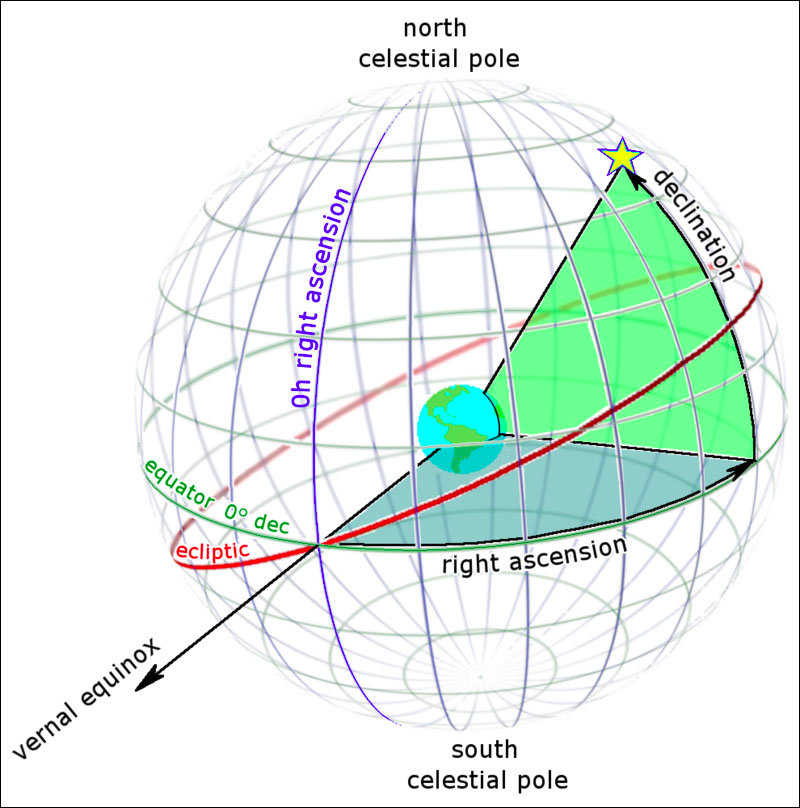
\includegraphics[width=0.9\textwidth]{figures/equatorial_system.png}
  \caption{Sistema de Coordenas Equatorial Geocêntrica. Fonte: Sky \& Telescope}
  \label{fig:coord-equatorial}
\end{figure}

A Esfera Celeste é umma esfera imaginária de raio arbitrário, centrada na Terra, sobre a qual os astros parecem estar fixados. A esfera celeste facilita a representação das coordenadas dos corpos celestes. O Plano do Equador Celeste é a projeção do plano equatorial da Terra na esfera celeste. Este plano divide a esfera celeste em dois hemisférios: norte e sul. Os Pólos Celestes são os pontos em que o eixo de rotação da Terra intercepta a esfera celeste. O Polo Norte Celeste está alinhado aproximadamente com a Estrela Polar.

A Ascensão Reta (\emph{Right Ascension}) é a medida angular ao longo do equador celeste, partindo do ponto vernal (ou ponto Áries), que é a interseção do equador celeste com a eclíptica (o caminho aparente do Sol no céu ao longo do ano). A ascensão reta é medida em horas, minutos e segundos, variando de 0 a 24 horas. Cada hora corresponde a 15 graus de arco.

A Declinação (\emph{Declination}) é a medida angular perpendicular ao equador celeste, indicando a distância de um objeto acima ou abaixo do equador. A declinação é expressa em graus, minutos e segundos de arco, variando de +90° no Polo Norte Celeste a -90° no Polo Sul Celeste.



\subsubsection{Análise dos Dados}
A compilação de um conjunto representativo de imagens astronômicas, abrangendo diferentes tipos de objetos celestes e fenômenos (por exemplo, galáxias espirais ou elípticas isoladas, sistema de galáxias em interação, galáxias irregulares, etc.) é altamente relevante para treinar um modelo com uma boa capacidade de generalização. %Assim, nesta etapa, é necessária uma análise preliminar dos dados para entender suas características e variações.





\subsection{Modelo de Aprendizagem Profunda}
\label{sec:modelo}
\subsubsection{Seleção da Arquitetura}
Uma etapa fundamental no desenvolvimento do modelo de aprendizagem profunda é a escolha de uma arquitetura de rede neural apropriada para a tarefa de geração de \emph{embeddings} visuais, como Redes Neurais Convolucionais (CNN, \cite{cnn}) ou Vision Transformers (ViT, \cite{ViT}).

\subsubsection{Pré-processamento dos Dados}
O pré-processamento envolve a implementação de técnicas de pré-processamento para normalização, redimensionamento e aumento dos dados, visando melhorar a qualidade e a diversidade dos dados de treinamento para garantir uma melhor capacidade de generalização do modelo.

\subsubsection{Treinamento}
\label{sec:treinamento}
O treinamento supervisionado do modelo de aprendizagem profunda usando o conjunto de treinamento preparado (Seção \ref{sec:preparacao}) contendo as imagens e os rótulos provenientes dos volutários. Nesta etapa, ocorre os ajustes de hiperparâmetros para otimizar o desempenho do modelo, sendo essencial para garantir a capacidade de generalização da rede neural e para evitar o subajuste ou o sobreajuste.

\subsubsection{Avaliação e Melhoria}
\label{sec:avaliacao}
A avaliação do modelo consiste em quantificar a capacidade preditiva do modelo utilizando métricas como precisão, recall e F1-score. Nessa etapa pode ocorrer a implementação de melhorias iterativas baseadas nos resultados obtidos.

\subsubsection{Inferência}
\label{sec:inferencia}
Após o treinamento (Seção \ref{sec:treinamento}) e avaliação (Seção \ref{sec:avaliacao}) do modelo, é possível utilizá-lo  no modo de inferêcia (ou predição) para geração dos \emph{embeddings} que serão armazenados na base de dados (Seção \ref{sec:db}).




\subsection{Banco de Dados e Algoritmos de Busca}
\label{sec:db}
\subsubsection{Design do Banco de Dados}
A estruturação do banco de dados é essencial para o armazenamento eficiente dos vetores (\emph{embeddings}). Atualmente, com o crescente uso de aprendizagem profunda nas aplicações, vários tipos de Sistema de Gerenciamento de Banco de Dados (SGBD) possuem suporte ao tipo de dado vetorial, essencial para o armazenamento dos \emph{embeddings}, incluindo os SGBD's relacionais, orientados a documentos e orientados a vetores. Desse modo, é importante considerar os aspectos de escalabilidade e desempenho para fazer a escolha do melhor SGBD.

\subsubsection{Indexação e Recuperação}
Os algoritmos e estruturas de dados relacionados a indexação de vetores em um banco de dados possuem grande impacto no tempo de inserção e recuperação dos dados. Por isso, é necessária uma escolha minusiosa do algoritmo de indexação dos \emph{embeddings} para permitir buscas rápidas e precisas por similaridade. Algumas estruturas de dados (e algoritmos) comumente usadas para esta finalidade são: Árvores k-dimensionais (KD-trees, \cite{kdtree}), \emph{Locality-Sensitive Hashing} (LSH, \cite{lsh}), \emph{Hierarchical Navigable Small World} (HNSW, \cite{hnsw}) e \emph{Inverted File Flat} (IVFFLAT, \cite{ivfflat}).

\subsubsection{Testes de Desempenho}
Para assegurar que o banco de dados e os algoritmos de busca atendam aos requisitos de tempo de resposta e escalabilidade, é essencial a realização de testes de carga e desempenho.


\subsection{Aplicação Web}
\label{sec:webapp}
\subsubsection{Design de Interface do Usuário}
Criação de \emph{wireframes} e protótipos da interface \emph{web}, focando na usabilidade e acessibilidade para os usuários finais.

\subsubsection{Implementação Front-end e Back-end}
Desenvolvimento da aplicação web utilizando frameworks modernos, como \texttt{React} (\url{www.react.dev}) para \emph{front-end} e \texttt{Django} (\url{www.djangoproject.com}) para \emph{back-end}, além da integração do sistema de busca com a interface \emph{web}.

\subsubsection{Testes de Usabilidade}
Realização de testes com usuários reais para coletar feedback sobre a interface e a experiência de uso e também da implementação de melhorias baseadas no feedback recebido.





\subsection{Sistema Inteligente para Descobertas em Astronomia}
\label{sec:sistema_inteligente}
\subsubsection{Integração dos Módulos}
\label{sec:integracao}
O sistema é composto pelos seguintes módulos: um modelo de aprendizagem profunda aplicado à visão computacional (Seção \ref{sec:modelo}), um banco de dados (Seção \ref{sec:db}) e uma aplicação \emph{web} (Seção \ref{sec:webapp}). Cada módulo tem sua funcionalidade específica dentro do sistema e será implementado de forma inedpendente. Isto é, os módulos poderão ser implementados paralelamente, aumentando o aproveitamento de tempo (conforme Fig. \ref{fig:cronograma}).

O \emph{design} de \emph{software} de cada módulo será feito de forma a garantir a integração contínua durante o desenvolvimento, perimitindo a realização testes fim-a-fim e correção de possíveis incompatibilidades entre os módulos previamente.




\subsubsection{Testes do Sistema}
\label{sec:validacao_final}
Os testes do sistema, ou testes fim-a-fim, tem como propósito garantir a qualidade e usabilidade do sistema como um todo, garantindo a interoperabilidade entre os seus módulos (descritos na Seção \ref{sec:integracao}) no ambiente de produção.



\subsection{Comparação dos resultados}
\label{sec:comparacao}
\subsubsection{Identificação dos Critérios de Comparação}
Selecionar os principais critérios de avaliação utilizados nos estudos de referência (Seção \ref{sec:revisao}), como métricas de desempenho (ex: precisão, recall, F1-score), eficiência computacional (ex: tempo de processamento, uso de recursos), e aplicabilidade prática (ex: facilidade de uso, escalabilidade).


\subsubsection{Coleta de Dados Comparativos}
Após o desenvolvimento do sistema, coletar os dados de desempenho obtidos em experimentos controlados, utilizando os mesmos conjuntos de dados ou similares aos utilizados nos estudos selecionados. Garantir que os experimentos sejam reproduzíveis e documentados de forma detalhada.


\subsubsection{Análise e Discussão}
A análise quantitativa consiste em comparar os resultados numéricos do sistema desenvolvido com os dados dos estudos de referência utilizando gráficos, tabelas e estatísticas descritivas para visualizar as diferenças e similaridades. Alguns exemplos incluem: 1) a precisão na classificação de objetos astronômicos, 2) o tempo de resposta para busca por similaridade visual e 3) a robustez e generalização do modelo em diferentes conjuntos de dados astronômicos.

Por outro lado, a análise qualitativa consiste em realizar uma comparação dos resultados, discutindo as vantagens e limitações do sistema em relação aos métodos existentes., considerando aspectos como inovação tecnológica, complexidade da implementação, e potencial de melhoria futura.

Finalmente, é importante elaborar uma discussão crítica e detalhada, identificando  possíveis discrepâncias entre os resultados obtidos e os apresentados nas referências bibliográficas (Seção \ref{sec:revisao}). Investigar as causas dessas discrepâncias, como diferenças nos conjuntos de dados, variações nos parâmetros dos modelos, ou melhorias implementadas no sistema proposto.






\section{Resultados Esperados}
\label{sec:resultados}
Tendo em vista os objetivos enunciados na Seção \ref{sec:metodologia}, o resultadado esperado é um sistema inteligente operante e funcional composto pelos seguintes módulos:
\begin{itemize}
  \item Um modelo de aprendizagem profunda em visão computacional treinado e capaz de gerar \emph{embeddings} a partir de imagens astronômicas.
  \item Um banco de dados para o armazenamento dos \emph{embeddings} gerados pelo modelo de aprendizagem profunda baseado em algum sistema gerenciador de banco de dados existente, otimizado para busca em milhões de vetores (\emph{embeddings}).
  \item Uma aplicação web intuitiva e dinâmica para realização das buscas.
\end{itemize}

Ao final do projeto, espera-se que o sistema desenvolvido não apenas atenda às necessidades imediatas de busca por similaridade visual em astronomia, mas também sirva como uma base para futuras inovações e melhorias em tecnologias de processamento e análise de imagens astronômicas. Assim, o sucesso deste projeto pode abrir novas possibilidades para a exploração do universo, além do avanço do conhecimento científico em outras áreas que enfrentam problemas similares de recuperação de informação semântica em imagens, como medicina, agricultura e geociências.





\section{Conclusão}
Nesta pesquisa, exploramos a eficácia de modelos de aprendizagem profunda para a tarefa de classificação de imagens em múltiplas campanhas do Galaxy Zoo. Inicialmente, discutimos a arquitetura do sistema inteligente e suas vantagens em lidar com tarefas de visão computacional, destacando sua capacidade de capturar informações locais e globais por meio de atenção multi-eixo. Além disso, abordamos técnicas de treinamento e regularização utilizadas para melhorar o desempenho e a generalização do modelo.


Uma interface web para consulta de imagens por similaridade oferece uma plataforma intuitiva e acessível para os usuários explorarem grandes conjuntos de dados visuais de maneira eficiente e eficaz. Ao permitir que os usuários busquem por uma imagem de consulta, essa interface utiliza algoritmos de busca por similaridade visual, como o HNSW, combinados com embeddings de modelos como o MaxViT, para recuperar imagens semelhantes a partir de um banco de dados vasto. Isso proporciona uma experiência de busca visualmente rica, onde os usuários podem descobrir imagens relacionadas com rapidez e precisão, facilitando tarefas como encontrar inspiração criativa, identificar objetos específicos ou explorar conceitos visuais.

Uma das principais vantagens de uma interface web para consulta de imagens por similaridade é sua acessibilidade universal. Ao fornecer uma plataforma baseada na web, os usuários podem acessar a ferramenta a partir de qualquer dispositivo conectado à Internet, incluindo computadores desktop, laptops, tablets e smartphones. Isso torna a busca por imagens por similaridade uma tarefa conveniente e flexível, permitindo que os usuários explorem conteúdo visual de forma intuitiva em qualquer lugar e a qualquer momento.

Em suma, os resultados obtidos até o momento são encorajadores, demonstrando o potencial do sistema inteligente para a criação de representações de imagens em conjuntos de dados astronômicos. No entanto, são necessárias análises adicionais e ajustes para garantir a eficácia e a robustez do modelo em diferentes cenários de aplicação. Futuros trabalhos podem se concentrar em investigar ainda mais as causas da queda no desempenho e explorar estratégias adicionais para melhorar a capacidade de generalização do modelo.





% \section{Infraestrutura}
% \label{sec:infra}
% Máquina virtual equipada com GPU's para o treinamento do modelo de aprendizagem profunda e uma máquina virtual para hosperagem da aplicação no ambiente de produção (presente no IAG).






\newpage
\section{Cronograma}
\label{sec:cronograma}
.

\begin{figure}[!ht]
  \centering
  \begin{ganttchart}[%
      x unit=0.88cm,
      y unit title=1.20cm,
      y unit chart=1.20cm,
      time slot format=isodate-yearmonth,
      time slot unit=month,
      vgrid={*1{draw=black!5, line width=.75pt}},
      group left shift=0,
      group right shift=0,
      group height=.15,
      group peaks tip position=0,
      group/.append style={fill=groupblue},
      bar/.append style={fill=barblue},
      milestone/.append style={fill=groupblue},
    ]{2024-1}{2024-12}
    \gantttitlecalendar{year,month=shortname} \ganttnewline

    \ganttgroup{Parte Técnica}{2024-1}{2024-11} \ganttnewline
    \ganttbar{Coleta de Dados (Seção \ref{sec:preparacao})}{2024-1}{2024-4} \ganttnewline
    \ganttbar{Modelo de DL (Seção \ref{sec:modelo})}{2024-5}{2024-8} \ganttnewline
    \ganttbar{Base de Dados (Seção \ref{sec:db})}{2024-8}{2024-10} \ganttnewline
    \ganttbar{Aplicação Web (Seção \ref{sec:webapp})}{2024-5}{2024-11} \ganttnewline
    \ganttbar{Integração \& Teste (Seção \ref{sec:sistema_inteligente})}{2024-1}{2024-11} \ganttnewline

    \ganttgroup{Parte Acadêmica}{2024-1}{2024-12} \ganttnewline
    \ganttbar{Rev. Literária (Seção \ref{sec:revisao})}{2024-1}{2024-3} \ganttnewline
    \ganttbar{Escrita da Dissertação}{2024-3}{2024-12} \ganttnewline
    \ganttbar{Revisão Contínua}{2024-5}{2024-12} \ganttnewline
    \ganttbar{Comp. Resultados (Seção \ref{sec:comparacao})}{2024-11}{2024-12} \ganttnewline

    \ganttmilestone{Submissão da Dissertação}{2024-12}
  \end{ganttchart}

  \caption{Cronograma de atividades\label{fig:cronograma}}
\end{figure}








% O \emph{Galaxy Zoo} \citep{galaxyzoo} é um projeto de ciência cidadã \citep{cs-bonney, cs-naturalscience} que insere a colaboração voluntária de membros da sociedade no processo de construção do conhecimento científico na área de astronomia. Ao decorrer de várias campanhas, o \emph{Galaxy Zoo} coletou milhões de classificações visuais humanas provenientes dos voluntários e que estão disponíveis para uso na ciência.


% Trabalhos anteriores utilizando modelos de \emph{Deep Learning} (DL) para classificar imagens astronômicas mostraram que é possível desenvolver modelos com grande capacidade preditiva usando as classificações dos voluntários como rótulos durante o treinamento supervisionado de redes neurais \citep{esnet, cs-ml}. Nesse sentido, o objetivo é usar as classificações provenientes do \emph{Galaxy Zoo} para realizar o treinamento do modelo de DL para ser a base de sistema inteligente capaz de recuperar informações visuais de imagens. Desse modo, a proposta deste projeto é desenvolver um sistema inteligente de busca por similaridade visual em grandes bases de imagens astronômicas, possuindo três principais funções: gerar representaçãoes visuais (Seção \ref{sec:modelo}), realizar buscas por similaridade visual (Seção \ref{sec:db}) e possibilitar a interação com o usuário por uma aplicação \emph{web} (Seção \ref{sec:webapp}). O sistema proposto tem o potencial de aprimorar a forma como os dados astronômicos são pesquisados e analisados, tornando a busca visual em dezenas de milhões de imagens um processo rápido, preciso e acessível. Além de contribuir no avanço do conhecimento científico para demais áreas que lidam com problemas similares, como sensoriamento remoto, medicina e agricultura.



% As galáxias estão em constante movimento e, quando muito próximas, são atraídas umas pelas outras. Nesta aproximação, elas podem interagir até se fundirem. A aproximação, a interação e a fusão entre galáxias representou um papel importante na evolução das galáxias durante a vida do universo. Visto que, neste processo, ocorre a troca de matéria entre as galáxias interagentes, vários fenômenos são desencadeados, como a formação de novas estrelas ou, até mesmo, a ativação do buraco negro no centro da galáxia, tornando-se um Núcleo Ativo de Galáxia (\emph{Active Galaxy Nuclei -- AGN}), devido ao fluxo de gás para o centro.

% Galáxias que estão no final desta cadeia de interação são morfologicamente classificadas como ``merger''. Esta classificação ainda pode ser dividida em outras duas subclassificações dependendo do estágio da fusão: \emph{pre-merger}, se for possível detectar visualmente as galáxias interagentes de forma independente e \emph{post-merger}, caso as galáxias já tenham se unido e for possível identificar apenas uma galáxia com distorções em sua estrutura.

% O final do século 20 foi marcado por uma revolução na maneira de se estudar galáxias na Astronomia quando os primeiros mapeamentos de grandes áreas do céu começaram a ser feitos. O mapeamento que mais impactou a Astronomia nas últimas décadas foi o \emph{Sloan Digital Sky Survey} (SDSS)\footnote{Website: \url{https://sdss.org}.} \citep{sdss17}. Com a necessidade de processar o grande volume de dados gerado por este levantamento, foi criado o GalaxyZoo\footnote{Website: \url{https://galaxyzoo.org}} \citep{galaxyzoo}, um programa de ciência cidadã (\emph{citizen science}) que envolveu o SDSS e milhares de cidadãos - ele foi realizado, em sua maioria, por pessoas sem vínculo acadêmico, que contribuíram com suas observações para a classificação morfológica de um grande número de galáxias do SDSS a partir da inspeção visual das imagens. A segunda liberação de dados do GalaxyZoo possui um catálogo com classificações morfológicas de trezentas mil galáxias, revisadas segundo o método de \cite{hart2016}. No presente trabalho, usamos classificações do GalaxyZoo para criar o conjunto de treinamento do modelo proposto.

% Com o avanço dos levantamentos astronômicos digitais (\emph{surveys}) e conseguinte aumento da quantidade de dados coletados, se torna crucial o desenvolvimento de métodos rápidos e automatizados para a classificação morfológica de galáxias sem a perda da acurácia da tradicional classificação visual \citep{yamauchi2005}. O uso do Aprendizado de Máquina (\emph{Machine Learning -- ML}) e, mais recentemente, do Aprendizado Profundo (\emph{Deep Learning -- DL}) tem mostrado resultados relevantes para problemas de classificação em diversos problemas nas áreas de visão computacional.

% O DL \citep{Goodfellow2016} é um segmento específico dentro da área de ML, por conseguinte, da área de Inteligência Artificial (IA). Consiste no desenvolvimento de Redes Neurais Artificiais que são combinadas em um número significativamente maior do que as redes neurais tradicionais. Este tipo de técnica se transformou no estado-da-arte do reconhecimento de padrões em imagens devido a um tipo específico de rede neural conhecida como convolucional. As Redes Neurais Convolucionais (\emph{Convolutional Neural Networks -- CNN}) \citep{lecun2015deep}, são inspiradas e propostas com certa analogia ao processamento das imagens realizadas no córtex visual de mamíferos. O processo começa quando um estímulo visual alcança a retina e equivale a um sinal que atravessa regiões específicas do cérebro. Essas regiões são responsáveis pelo reconhecimento de cada uma dessas características correspondentes \citep{karpathy2016convolutional}. Os neurônios biológicos das primeiras regiões respondem pela identificação de formatos geométricos primários, enquanto neurônios das camadas finais têm a função de detectar características mais complexas, formadas pelas formas simples anteriormente reconhecidas \citep{vedaldi2015matconvnet}. Características com padrões muito específicos do objeto são estabelecidas depois que o procedimento se repete. De forma análoga, a CNN decompõe a tarefa de reconhecimento de um objeto em subtarefas. Para isso, durante a aprendizagem, a CNN divide a tarefa em subníveis de representação das características, posteriormente aprendendo a reconhecer novas amostras da mesma classe \citep{lecun2015deep, vedaldi2015matconvnet}. Desta forma, as CNNs são capazes de predizer características complexas sem a necessidade de um pré-processamento e são invariantes à escala e à rotação dos dados, o que as torna essenciais na classificação em imagens.

% Os transformadores representam uma classe de arquiteturas de aprendizado de máquina que revolucionaram o campo da inteligência artificial, particularmente em tarefas relacionadas ao processamento de linguagem natural e visão computacional. Sua abordagem inovadora de processamento baseado em atenção, introduzida pelo modelo original Transformer, permitiu capturar relações complexas e de longo alcance entre os elementos de uma sequência, sem depender de arquiteturas convolucionais. A capacidade dos transformadores de modelar dependências contextuais em dados sequenciais tornou-os altamente adaptáveis a uma variedade de tarefas, desde tradução automática e geração de texto até reconhecimento de objetos e análise de imagens.

% A aplicação dos princípios dos transformadores \cite{vaswani2017attention} ao campo da visão computacional deu origem a arquiteturas como o Vision Transformer (ViT) \cite{ViT}, que representam uma abordagem inovadora para análise de imagens. O ViT trata imagens como sequências de patches e aplica diretamente mecanismos de atenção para capturar relações espaciais e semânticas entre eles. Essa abordagem tem se mostrado altamente eficaz, rivalizando com as tradicionais redes neurais convolucionais em uma variedade de tarefas de visão, destacando o potencial dos transformadores como uma ferramenta poderosa e versátil em domínios além do processamento de linguagem natural.

% As representações geradas pelo modelo de ViT representam uma poderosa base de conhecimento em visão computacional, capturando de forma compacta e semântica as características visuais essenciais das imagens. Esses embeddings, obtidos através do processo de codificação realizado pelo ViT, encapsulam informações valiosas sobre a estrutura e o conteúdo das imagens, possibilitando uma representação rica e abstrata do espaço visual. Essa base de conhecimento baseada em deep learning oferece uma maneira eficaz de entender e comparar visualmente as imagens, permitindo uma ampla gama de aplicações, desde a recuperação de imagens até a análise de similaridade visual em conjuntos de dados complexos.

% Ao utilizar os embeddings do ViT para busca por similaridade visual, podemos explorar as relações semânticas e visuais entre as imagens de uma maneira intuitiva e eficiente. Essa abordagem aproveita a capacidade do ViT de capturar informações contextuais e hierárquicas nas imagens, permitindo uma representação robusta e discriminativa do espaço visual. Ao calcular a similaridade entre os embeddings, podemos identificar padrões visuais comuns, descobrir relações semânticas entre imagens e realizar uma recuperação eficaz de imagens com base em critérios visuais específicos.

% Além disso, a base de conhecimento construída a partir dos embeddings do ViT tem o potencial de impulsionar uma variedade de aplicações em visão computacional, incluindo reconhecimento de objetos, classificação de imagens e análise de conteúdo visual. Ao fornecer uma representação densa e semântica das imagens, os embeddings do ViT podem servir como uma fonte de informações valiosa para sistemas de recomendação, indexação de imagens e pesquisa visual em larga escala. Essa base de conhecimento baseada em deep learning tem o potencial de transformar fundamentalmente a forma como interagimos com as imagens, permitindo uma compreensão mais profunda e sofisticada do conteúdo visual em diferentes domínios de aplicação.


% \section{Conjuntos de Dados}
% \label{sec:conjunto_dados}
% \subsection{Coleção de Imagens, Catálogos e Rótulos}
% \label{sec:imagens_catalogos_rotulos}
% As imagens são as principais entradas do modelo - é a partir delas que são feitas as classificações morfológicas. As imagens foram obtidas através do Legacy Survey DR10 nas bandas G, R e I.

% Os catálogos são tabelas liberadas pelos próprios levantamentos astronômicos contendo propriedades físicas dos objetos medidas a partir de fotometria ou espectroscopia. Foram usados dois catálogos: Legacy Survey DR10, contendo fotometria, e SDSS DR17, contendo espectroscopia.

% E, por fim, os rótulos são as classificações morfológicas feitas a partir de inspeção humana ou automática. São eles que definem a classe de cada objeto no conjunto. Foram usadas classificações feitas por astrônomos \citep{darg-a, darg-b}, por voluntários (citizen science) \citep{gz1} e automáticas (aprendizagem profunda) \citep{gzdecals}.



% \subsection{Conjunto de Treino}
% \label{sec:conjunto_treino}
% O modelo proposto é treinado de forma supervisionada, ou seja, durante o treino, é necessário informar ao modelo a imagem da galáxia e seu respectivo rótulo. Sendo assim, o conjunto de treino é composto pelas imagens e seus respectivos rótulos. A seguir são descritas a formação de cada classe, bem como do conjunto de treino completo.


% \subsubsection{Classe Posistiva}
% \label{sec:classe_positiva}
% A classe positiva é constituída por galáxias mergers. Estas galáxias foram obtidas a partir de diversos catálogos, são eles:

% \begin{enumerate}
%     \item Classificações humanas do GalaxyZoo Decals DR5, feitas por voluntários \citep{gzdecals};
%     \item Classificações automáticas do GalaxyZoo Decals DR5, feitas por um modelo de DL \citep{gzdecals};
%     \item GalaxyZoo DR1, constituído por inspeção visual de voluntários \citep{gz1};
%     \item GalaxyZoo DR2, constituído por inspeção visual de voluntários \citep{hart2016};
%     \item Catálogo de galáxias mergers de \cite{darg-a, darg-b}, constituído por classificações feitas pelos autores do trabalho e pelo modelo criado por eles;
%     \item Busca do banco de dados do DR17 do SDSS \citep{sdss17} por objetos com magnitude na banda r e redshift similares; 
%     \item Busca por similaridade visual usando CNN pré-treinada (Seção \ref{sec:exploracao_conjunto_busca}).
%     \item Expansão do conjunto de dados do GalaxyZoo Decals
% \end{enumerate}

% Para selecionar os objetos dos itens 1, 2, 3 e 4, foi feita uma restrição para objetos com fração de votos maior que 0.85 para a classe merger (\texttt{merging\_merger\_fraction} $> 0.85$). No item 5, apenas os objetos com estágio de mesclagem (ver \cite{darg-b}) maior ou igual a 3 (\texttt{stage} $\ge 3$) foram selecionados. No item 6, foi buscado por todos os pares de objetos com distância angular menor que 0.5 arcmin, ambos com espectroscopia, que possuíssem diferença de redshift menor que 0.01 e diferença de magnitude na banda r menor que 1.5. E, no item 7, os objetos foram encontrados por similaridade visual das imagens do Conjunto de Busca tendo como base os objetos coletados nos itens 1 ao 6. Esse procediomento é melhor detalhado na Seção \ref{sec:exploracao_conjunto_busca}. O obtenção dos objetos pelo item 8 conta com auxilio de vários diagramas para fazer uma seleção no conjunto de dados do GalaxyZoo Decals. Uma pequena amostra de cada um desses itens é mostrada nas Figs. \ref{fig:img_grid_mergers} e \ref{fig:more_mergers}

% \begin{figure}[!ht]
%   \centering
%   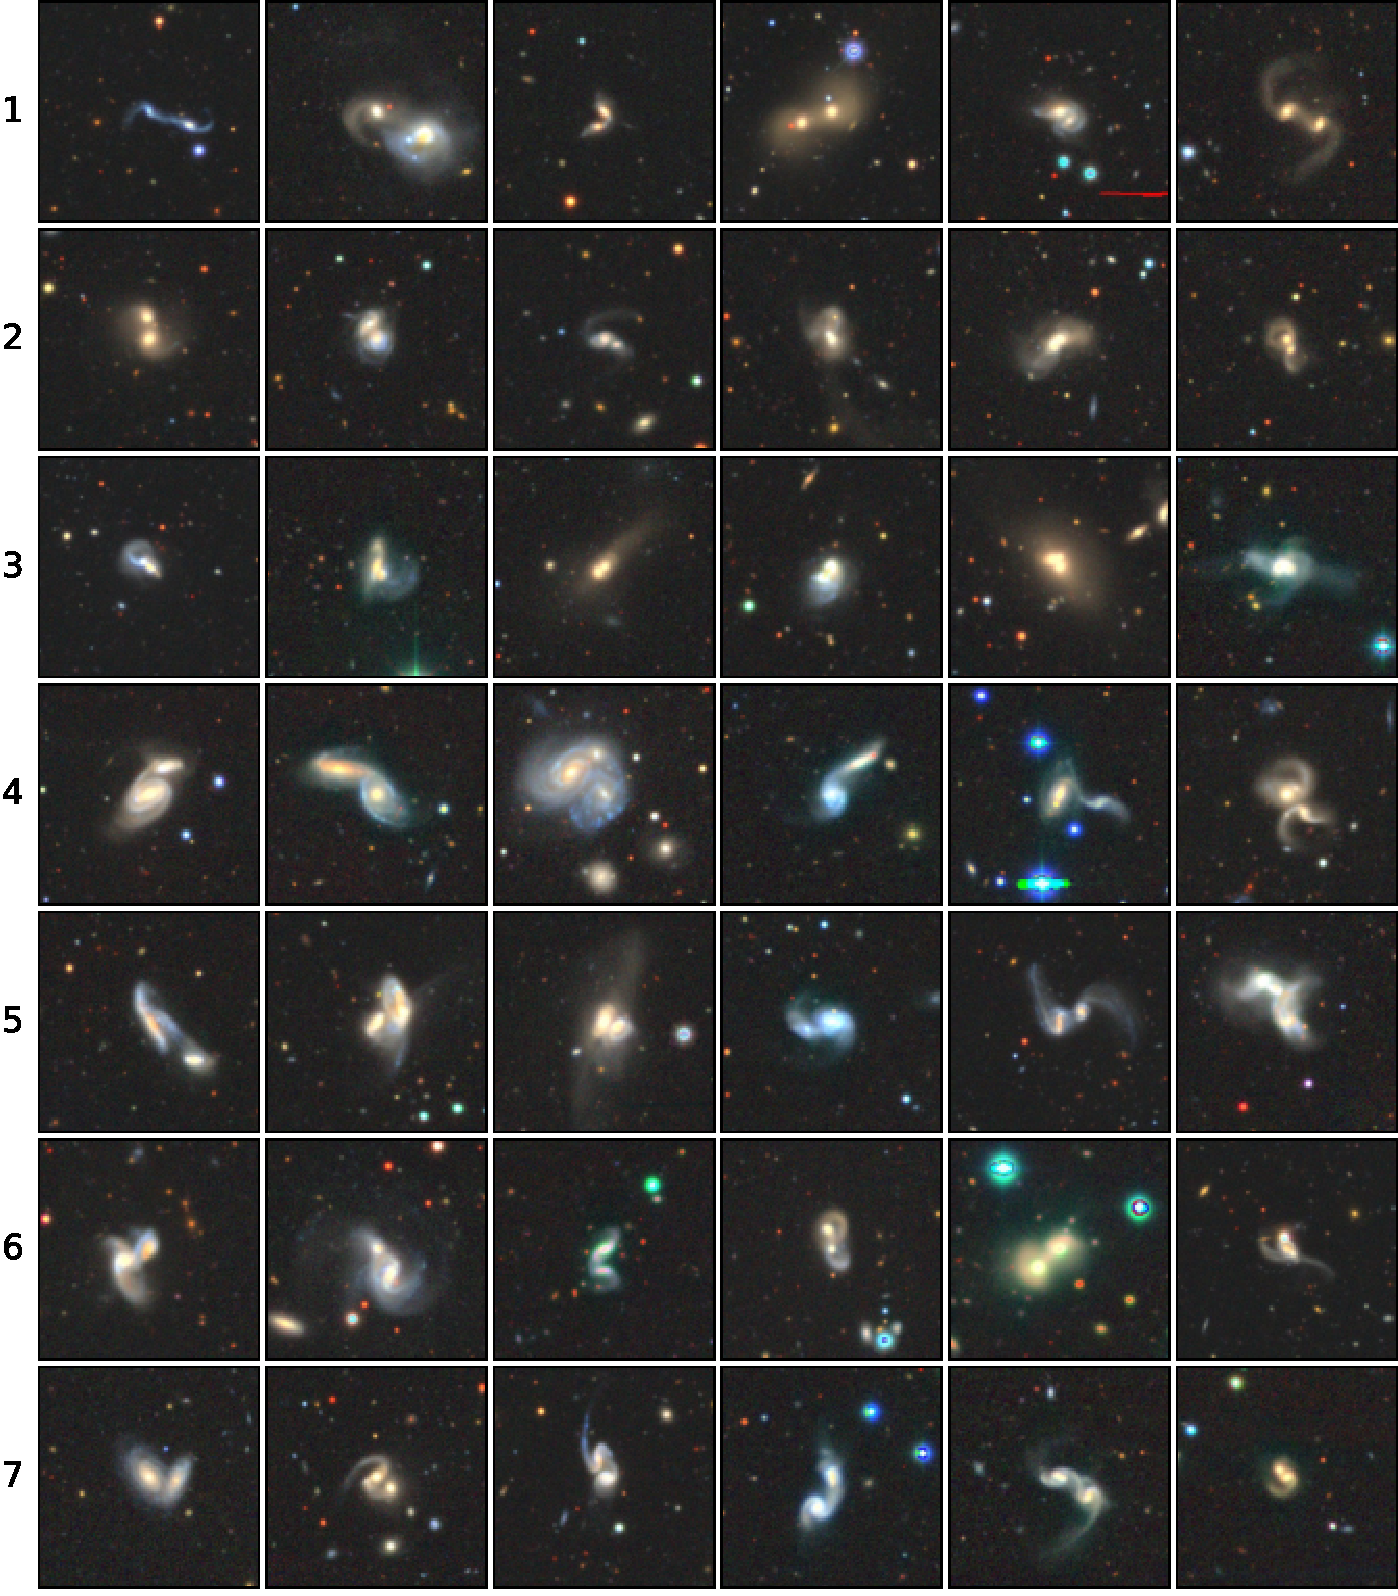
\includegraphics[width=\textwidth]{figures/img_grid_mergers.pdf}
%   \caption{Visualização de uma amostra de galáxias do conjunto de treino. As linhas 1 e 2 contêm objetos do catálogo GalaxyZoo Decals, constituído por classificações humanas e automáticas, respectivamente \citep{gzdecals}. A linha 3 possui objetos do catálogo de \citep{darg-a, darg-b}. As linhas 4 e 5 são compostas por objetos do DR1 e DR2 do GalaxyZoo, respectivamente \citep{gz1, hart2016}. A linha 6 contém objetos da busca no banco de dados do SDSS. Por fim, a linha 7 possui objetos encontrados a partir do Conjunto de Busca (\ref{sec:conjunto_busca}) pelo método descrito na Seção \ref{sec:exploracao_conjunto_busca}.}
%   \label{fig:img_grid_mergers}
% \end{figure}

% \begin{figure}[!ht]
%   \centering
%   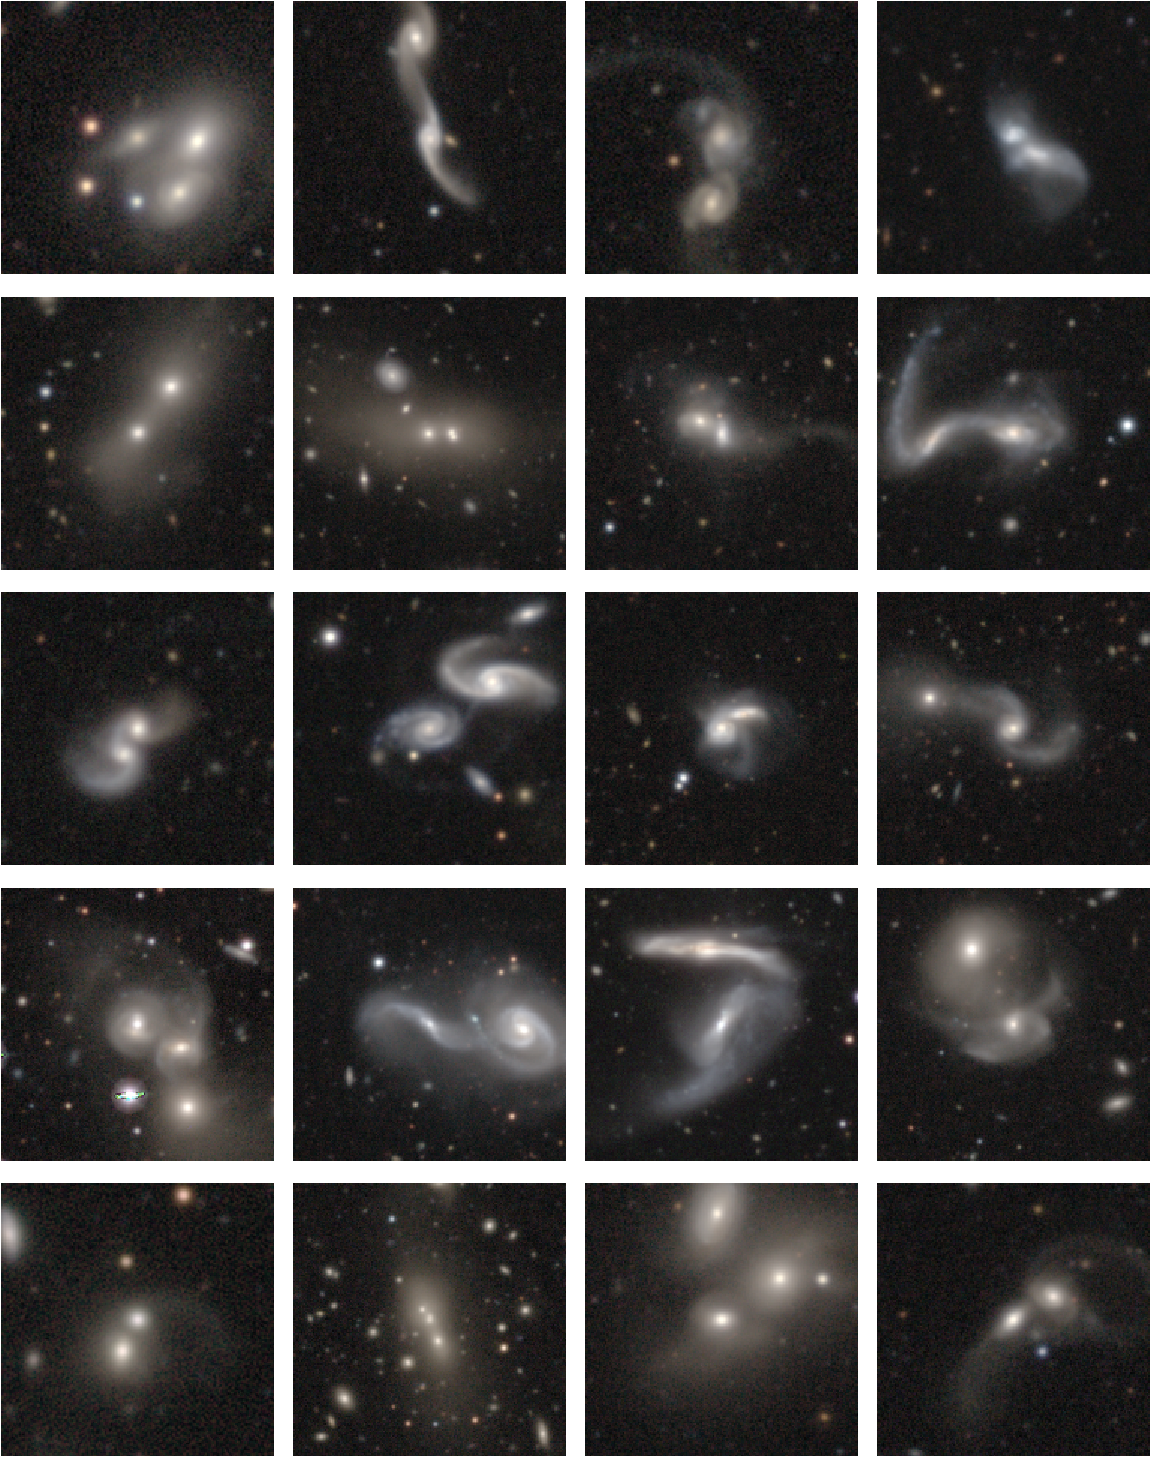
\includegraphics[width=\textwidth]{figures/blind_stamps_1.pdf}
%   \caption{Amostra do conjunto expandido do Galaxy Zoo Decals (oitavo item da lista)}
%   \label{fig:more_mergers}
% \end{figure}

% \newpage
% \subsubsection{Classe Negativa}
% \label{sec:classe_negativa}
% A classe negativa é composta por objetos que não sejam galáxias mergers. Esta classe tenta generalizar o exemplo negativo de uma galáxia merger, sendo composta por objetos de diferentes tipos. As seguintes fontes foram usadas:

% \begin{enumerate}
%     \item Galáxias Elípticas e Espirais do DR1 do GalaxyZoo;
%     \item Galáxias Elípticas, Espirais e S0 do DR2 do GalaxyZoo;
%     \item Busca por conjunto estrela-galáxia no banco de dados do DR17 do SDSS;
%     \item Busca por objetos espectrospicamente classificados como estrela no banco de dados do SDSS DR17.
% \end{enumerate}

% Os itens 1 e 2 foram feitos a partir da adição das restrições de que o objeto deve ter uma fração de votos maior que 0.85 para cada uma das morfologias (Elíptica, Espiral ou Lenticular) e menor que 0.05 para classe merger. O item 3 foi obtido a partir da consulta por todos os objetos espectroscopicamente classificados como galáxias com distância angular menor que 0.5 arcmin de um objeto espectroscopicamente classificado como estrela no banco de dados do SDSS DR17. O item 4 comtém apenas objetos classificados como estrela no banco de dados do SDSS DR17. 


% \subsubsection{Composição Final}

% O Conjunto de Treino é composto pelas seleções dos objetos descritas para a classe positiva (Seção \ref{sec:classe_positiva}) e negativa (Seção \ref{sec:classe_negativa}). Durante a união das amostras para formar este conjunto, todas as tabelas foram correlacionadas entre si para garantir que nenhum objeto tenha algum vizinho com uma distância angular menor que o campo de visão de cada imagem ($\approx$ 75 arcsec) para certificar de que o conjunto não tenha objetos duplicados.

% As imagens do Conjunto de Treino são divididas em duas classes: positiva e negativa, os objetos pertencentes à primeira classe são rotulados como ``merger'' e os pertencentes à segunda classe são rotulados como ``não-merger''. Todos os objetos, de ambas as classes, foram restringidos ao intervalo de magnitude na banda r de 15 a 18.5. Apenas a magnitude do objeto central foi restringida, com excessão das restrições que impuseram uma diferença de magnitude máxima entre o objeto central e o objeto vizinho. Estes valores foram decididos após a inspeção visual de uma parte do Conjunto de Treino. Foi notado que valores de magnitude menores que 15 aumentariam a quantidade de objetos para classificação, sendo que poucos deles seriam mergers; e, para valores maiores que 18.5, os detalhes dos objetos começam a ficar muito fracos, aumentando a incerteza da classificação. Além disso, todos as amostras selecionadas passaram por inspeção visual, onde algumas imagens foram retiradas. 

% \begin{figure}[!ht]
%   \centering
%   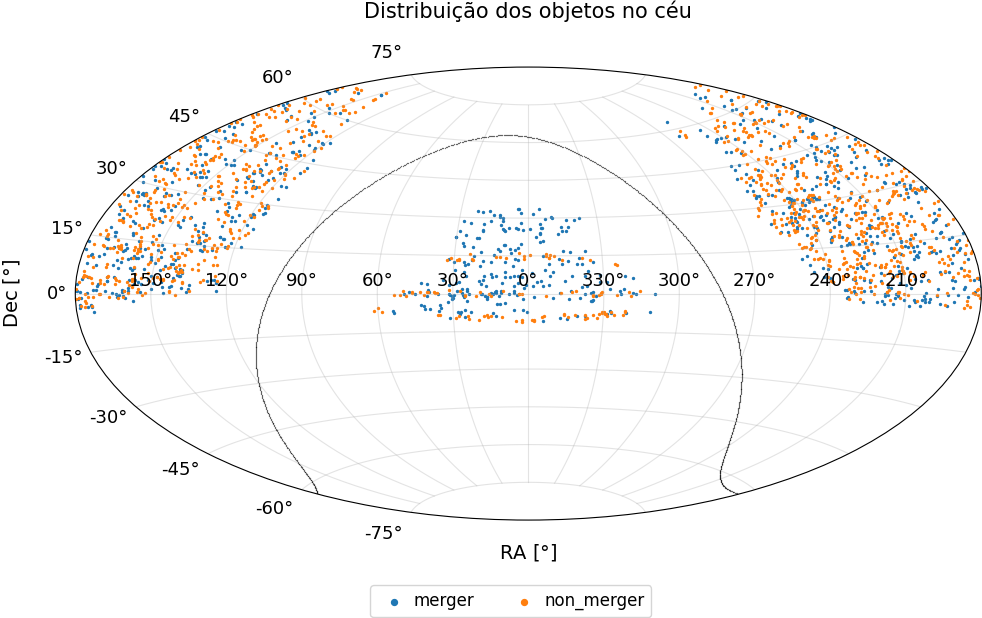
\includegraphics[width=.92\textwidth]{figures/sky_plot.png}
%   \caption{Posição espacial dos objetos do Conjunto de Treino. Em azul, as galáxias rotuladas como mergers, e, em laranja, as não-mergers}
%   \label{fig:sky_distrib}
% \end{figure}

% A Tabela \ref{tab:conjunto_treino} mostra a quantidade de objetos do Conjunto de Teste separadas por rótulo e fonte. Este conjunto é composto por 1702 galáxias rotuladas como mergers e 1780 objetos rotulados como não merger, totalizando 3482 objetos. A posição espacial desses objetos estão dispostos na Fig. \ref{fig:sky_distrib}.

% \begin{htable}{c|X|c|c}{Composição do Conjunto de Treino}{\bf Rótulo & \bf Fonte & \bf Objetos & \bf Total}{tab:conjunto_treino}
%     \multirow{6}{*}{Merger} & GZ Decals DR5 \citep{gzdecals} & 802 & \multirow{6}{*}{1702}\\
%     {} & \cite{darg-a, darg-b} & 168 & {}\\
%     {} & GZ DR 1 \citep{gz1} & 238 & {}\\
%     {} & GZ DR 2 \citep{hart2016} & 22 & {}\\
%     {} & SDSS DR17 \citep{sdss17} & 234 & {}\\
%     {} & Conjunto de Busca & 138 & {}\\
%     \hline
%     \multirow{5}{*}{Não-Merger} & Galáxias Elípticas \citep{gz1, hart2016} & 614 & \multirow{5}{*}{1780}\\
%     {} & Galáxias Espirais \citep{gz1, hart2016} & 680 & {}\\
%     {} & Galáxias Lenticulares \citep{hart2016} & 98 & {}\\
%     {} & Par Estrela-Galáxia & 278 & {}\\
%     {} & Estrelas & 110 & {}\\
% \end{htable}




% \subsection{Conjunto de Validação}
% \label{sec:conjunto_validacao}
% O modelo é avaliado usando validação cruzada \emph{k-fold}. Este método consiste em dividir o Conjunto de Treino (Seção \ref{sec:conjunto_treino}) em $k$ subconjuntos mutuamente exclusivos e de mesmo tamanho e, então, um subconjunto é utilizado para teste e os $k-1$ restantes são utilizados para estimação dos parâmetros. Este processo é realizado $k$ vezes alternando o subconjunto de teste de forma circular. Ao final das $k$ iterações, quando cada elemento do Conjunto de Treino já foi usado como validação uma única vez, calcula-se as métricas quantitativas de avaliação do modelo.


% \subsection{Conjunto Cego}
% \label{sec:conjunto_cego}
% O conjunto cego é formado por $\approx 100.000$ galáxias aleatórias no hemisfério sul sem classificação morfológica. O objetivo deste conjunto é ser usado para encontrar novas galáxias em interação usando o modelo com imagens classificadas no hemisfério norte do céu. Este conjunto é formado apartir de imagens do Legacy Survey DR10. A Fig. \ref{fig:blind_sample_sky} mostra a distribuição dos objetos neste conjunto no céu.

% \begin{figure}[!ht]
%     \centering
%     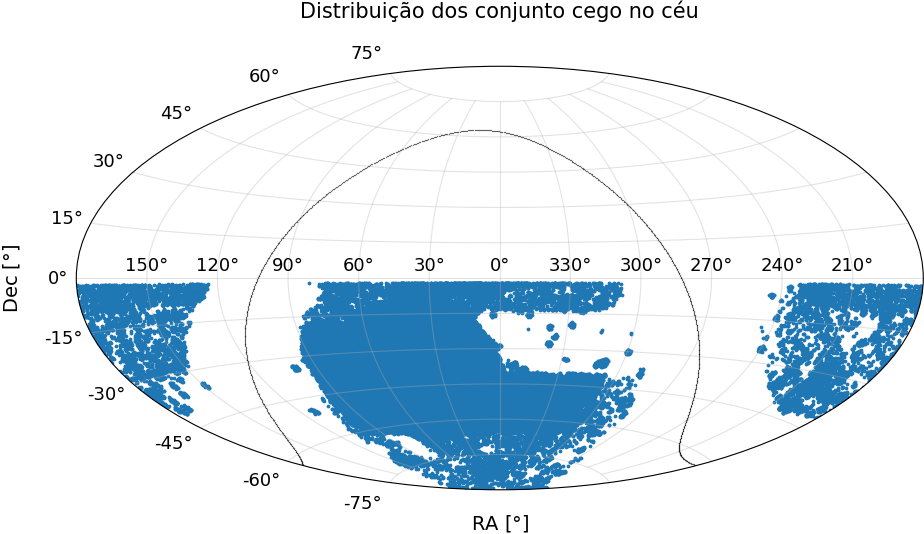
\includegraphics[width=\linewidth]{figures/blind_sample_sky}
%     \caption{Distribuição das galáxias do conjunto cego no céu}
%     \label{fig:blind_sample_sky}
% \end{figure}

% A seleção dos objetos para este conjunto foi feita a partir de uma amostragem aleatória no catálogo do DR10 do Legacy Survey para objetos que correspondessem às seguintes restrições:

% \begin{equation*}
%     \begin{cases}
%         \mathrm{dec} < -2\\
%         \mathrm{type} \neq \mathrm{PSF}\\
%         14 < \mathrm{mag\_r} < 19
%     \end{cases}
% \end{equation*}


% \subsection{Conjunto de Busca}
% \label{sec:conjunto_busca}

% \begin{figure}[!ht]
%   \centering
%   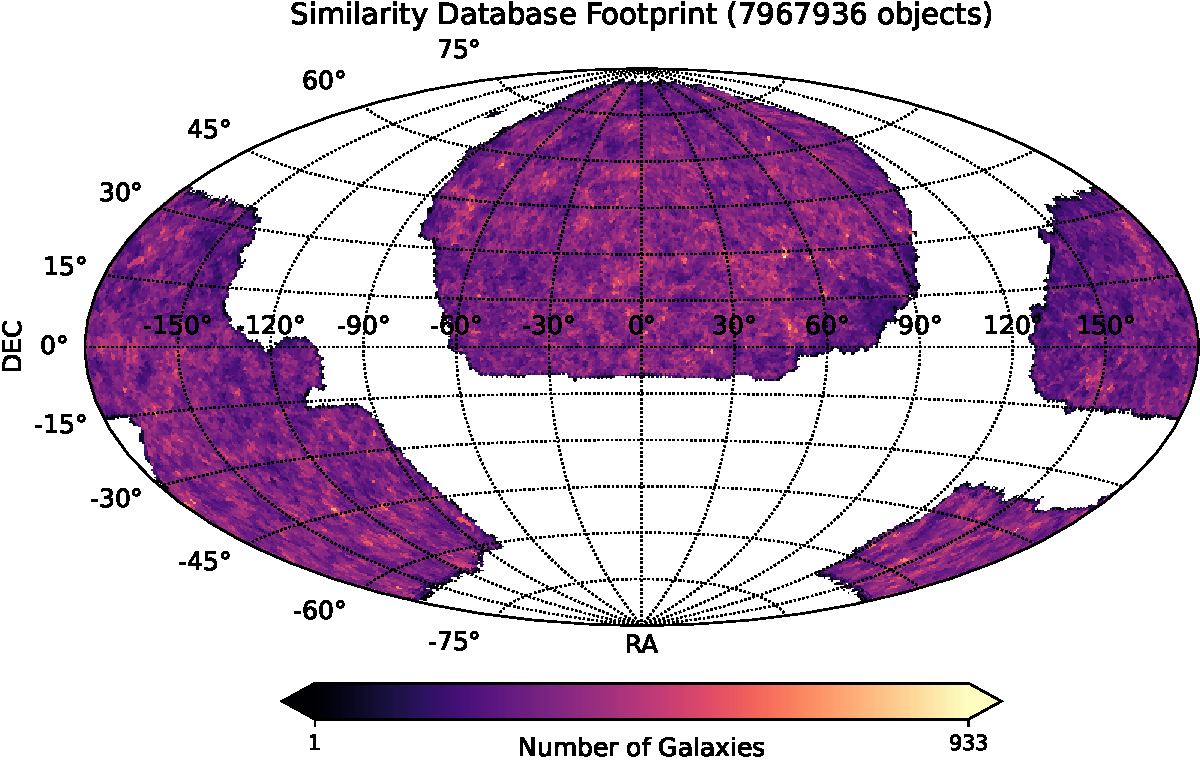
\includegraphics[width=\textwidth]{figures/similarity_footprint.pdf}
%   \caption{Disposição espacial (footprint) do conjunto de busca. A cor indica a densidade de objetos em uma determinada região.}
%   \label{fig:similarity_footprint}
% \end{figure}

% O conjunto de busca consiste em um repositório de 7.967.936 imagens que serão comparadas com uma imagem de consulta (query) para encontrar as imagens mais semelhantes com base nos \emph{embeddings} gerados pelo modelo. Este conjunto contém todas as imagens que serão comparadas quando uma nova imagem de consulta for apresentada. Estas são imagens de objetos que cobrem uma ampla gama de variações esperadas em termos de conteúdo visual. A Fig. \ref{fig:similarity_footprint} mostra a disposição espacial dos objetos.

% A principal finalidade do conjunto de busca é permitir a comparação por similaridade. Quando uma nova imagem de consulta é fornecida, seu embedding é comparado com os embeddings das imagens no conjunto de busca. As imagens cujos embeddings estão mais próximos (segundo uma métrica de distância, como a distância euclidiana ou coseno) são retornadas como resultados mais similares. O procedimento de busca é detalhado na Seção \ref{sec:exploracao_conjunto_busca}.



% A seleção dos objetos para este conjunto foi feita a partir de uma amostragem aleatória no catálogo do DR10 do Legacy Survey para objetos que correspondessem às seguintes restrições:

% \begin{equation*}
%   \begin{cases}
%     \mathrm{type} \neq \mathrm{PSF} \\
%     14 < \mathrm{mag\_r} < 17.77
%   \end{cases}
% \end{equation*}






% \section{Machine Learning \& Deep Learning}
% \subsection{Background}
% Aprendizagem de Máquina, \emph{Machine Learning -- ML}, é um campo da Inteligência Artificial que se concentra no desenvolvimento de algoritmos e técnicas que permitem que sistemas computacionais aprendam e melhorem com base em dados. O conceito por trás do Machine Learning existe há décadas, mas ganhou destaque significativo nas últimas duas décadas devido ao aumento na disponibilidade de dados, avanços em algoritmos e o poder de processamento computacional.

% O termo \emph{Machine Learning} foi definido como ``o campo de estudo que dá aos computadores a habilidade de aprender sem serem explicitamente programados'' por \cite{ml}. No entanto, os fundamentos do aprendizado de máquina remontam ainda mais, com raízes na estatística e na teoria da decisão.

% Já a Aprendizagem Profunda, \emph{Deep Learning -- DL}, é uma subárea da Aprendizagem de Máquina que se concentra em algoritmos inspirados na estrutura e funcionamento do cérebro humano, conhecida como Rede Neural Artificial (RNA). O termo ``profundo'' foi inserido devido à estrutura de várias camadas das Redes Neurais Artificiais, onde cada camada extrai características complexas dos dados de entrada, permitindo a construção de representações hierárquicas.

% O DL foi popularizado mais recentemente juntamente com o avanço da capacidade computacional cada vez maior, pois, usualmente, estes algoritmos demandam mais recursos computacionais que os algoritmos de ML clássicos.

% \subsection{Algoritmo k-NN}
% O algoritmo k-NN (k-Nearest Neighbors) é um método de aprendizado de máquina utilizado para classificação e regressão \citep{knn}. Ele é considerado um algoritmo de aprendizado supervisionado, pois utiliza um conjunto de dados de treinamento com rótulos conhecidos para realizar previsões ou classificações em novos dados. O k-NN é uma abordagem simples, mas poderosa, que consegue determinar a semelhança dos exemplos a partir do cálculo da proximidade no espaço de características a partir de métricas de distância, como a euclidiana ou a Manhattan, por exemplo %\cite{}.

% O funcionamento básico do algoritmo k-NN consiste em encontrar os $k$ vizinhos mais próximos de um ponto de consulta (exemplo a ser classificado). A proximidade é determinada por uma métrica de distância, geralmente a distância euclidiana, que mede a diferença entre as características do ponto de consulta e as características dos pontos no conjunto de treinamento. Uma vez que os $k$ vizinhos mais próximos são identificados, a classificação ou previsão do ponto de consulta é determinada pela maioria das classes dos vizinhos (no caso de classificação) ou pela média dos valores dos vizinhos (no caso de regressão).

% O algoritmo k-NN foi criado para resolver problemas de classificação e regressão em campos como reconhecimento de padrões, mineração de dados e análise de dados. Ele é especialmente útil quando a relação entre as características e as classes ou valores de saída não é facilmente modelada por uma equação matemática complexa. Em vez disso, o k-NN se beneficia de informações diretas dos dados de treinamento para fazer previsões ou classificações \citep{knn}.

% Este algoritmo é usado para resolver uma variedade de problemas, como classificação de documentos \citep{knn_docs}, recomendação de produtos \citep{knn_recomendations}, diagnóstico médico \citep{knn_biomed}, classificação de imagens \citep{knn_cv}, previsão de preços e valores \citep{knn_prices}, análise de sequências de DNA \citep{knn_dna}, etc.

% \subsection{Redes Neurais Convolucionais}
% \label{sec:cnn_def}
% As CNNs são um tipo de arquitetura de rede neural que foram desenvolvidas especialmente para tarefas de visão computacional, como classificação de imagens, detecção de objetos e segmentação de imagens \citep{lecun1989, lecun1998}. Essas redes são inspiradas no córtex visual do cérebro humano e são projetadas para processar imagens como entradas.

% As CNNs são compostas por várias camadas, incluindo camadas convolucionais, de \emph{pooling} e totalmente conectadas. As camadas convolucionais são responsáveis por extrair características importantes das imagens, como bordas, texturas e formas, enquanto as camadas de pooling são responsáveis por reduzir a dimensionalidade das características extraídas. As camadas totalmente conectadas são responsáveis por fazer a classificação final das imagens \citep{CholletBook}.

% Uma das principais vantagens é a capacidade de extrair características relevantes das imagens de forma automatizada, sem a necessidade de recursos humanos para a extração manual. Elas também são capazes de precessar imagens de diferentes tamanhos e resoluções, o que as torna flexíveis para trabalhar em diferentes tarefas. Além disso, ainda são capazes de aprender a partir de grandes conjuntos de dados e geralmente apresentam um desempenho superior em tarefas de classificação de imagens em comparação com outras arquiteturas de redes neurais. Isso se deve ao fato de que as CNNs são capazes de capturar informações locais e espaciais das imagens, o que é crucial para tarefas de visão computacional.

% % \subsection{EfficientNet}
% % \label{sec:efficientnet}
% % A arquitetura EfficientNet \citep{EfficientNet} foi desenvolvida como uma resposta à questão de como escalar modelos de convolução. Foram considerados três diferentes aspectos: profundidade, largura e resolução da imagem de entrada. Em vez de dimensionar cada aspecto manualmente, o modelo implementa um escalonamento composto que equilibra os aspectos para obter melhor desempenho, com isso a rede consegue uma alta acurácia usando muito menos parâmtros e operações de ponto flutuante por segundo (\emph{FLOPS}). Esta rede já foi usada na classificação de doenças em vegetais \citep{EfficientNetEx03}, eletrocardiogramas \citep{EfficientNetEx01} e cristalização de proteínas \citep{EfficientNetEx02}.


% \subsection{Vision Transformers (ViT)}
% O Vision Transformer (ViT) \citep{ViT} é uma arquitetura de aprendizagem profunda projetada para tarefas de visão computacional, inspirada no Transformer \citep{vaswani2017attention}, um modelo originalmente desenvolvido para processamento de linguagem natural (NLP). A principal inovação do ViT é a aplicação direta da arquitetura Transformer em imagens, sem a necessidade de convoluções, que são o alicerce das Redes Neurais Convolucionais (CNNs). O ViT trata uma imagem como uma sequência de patches, análoga à maneira como o Transformer trata sequências de palavras em NLP como sequência de tokens. Cada imagem é dividida em patches de tamanho fixo, que são achatados e linearmente embutidos em vetores de dimensão fixa, que são então processados pelo ViT.

% O funcionamento do Vision Transformer começa com a divisão da imagem de entrada em patches, geralmente de 16x16 pixels, que são convertidos em uma sequência de vetores de embeddings. Cada embedding representa um patch da imagem, e esses embeddings são enriquecidos com informações de posição para manter a noção de localização espacial dos patches. Esses vetores são então alimentados em um encoder Transformer, composto por múltiplas camadas de atenção e feed-forward. A atenção, especificamente a multi-head self-attention, permite que o modelo aprenda relações entre diferentes patches da imagem, capturando tanto informações locais quanto globais.

% Uma vez que os embeddings passam pelas camadas de atenção e feed-forward do encoder, o ViT agrega a informação de todos os patches para formar uma representação global da imagem. A atenção auto-regressiva do Transformer permite que o modelo foque em diferentes partes da imagem de forma dinâmica, adaptando-se às características visuais presentes. A camada final geralmente é uma camada de classificação, que utiliza a representação global da imagem para prever classes em tarefas de classificação de imagem. O ViT tem mostrado desempenho competitivo com as CNNs tradicionais em várias tarefas de visão, muitas vezes superando-as em cenários onde há uma abundância de dados de treinamento.

% Uma vantagem notável do Vision Transformer é sua capacidade de escalar eficientemente com dados. Enquanto as CNNs podem se tornar ineficientes e complexas com o aumento do tamanho da rede e da quantidade de dados, os Transformers são conhecidos por seu desempenho superior em grandes conjuntos de dados, devido à sua habilidade de modelar dependências de longo alcance e capturar interações complexas entre patches. No entanto, o treinamento eficaz do ViT requer grandes volumes de dados e recursos computacionais substanciais, o que pode ser uma limitação em alguns cenários. Em suma, o Vision Transformer representa uma abordagem inovadora e poderosa para tarefas de visão computacional, aproveitando os pontos fortes da arquitetura Transformer para superar algumas das limitações das redes convolucionais tradicionais.


% \subsection{MaxViT}
% A arquitetura MaxViT \citep{MaxViT}, que se refere ao Multi-axis Vision Transformer, é uma arquitetura recente na área de visão computacional que combina a eficiência das convoluções com a capacidade dos Transformers de modelar dependências de longo alcance. O MaxViT se distingue por seu uso de atenção multi-eixo, onde a atenção é aplicada em diferentes eixos (horizontal e vertical) em várias escalas. Isso permite uma captura mais eficaz e detalhada das características da imagem em diferentes dimensões e níveis de granularidade.

% O funcionamento da MaxViT começa com a divisão da imagem de entrada em patches, semelhante ao Vision Transformer (ViT). Esses patches são inicialmente processados por camadas convolucionais para extrair características locais e reduzir a resolução espacial da imagem. A partir daí, os patches são tratados como tokens e processados através de uma série de blocos de atenção multi-eixo. Em cada bloco, a atenção é aplicada separadamente ao longo dos eixos horizontal e vertical, o que permite ao modelo capturar padrões e relações em diferentes direções.

% A especificidade da MaxViT reside na sua estrutura de atenção multi-eixo, que proporciona uma visão mais detalhada e rica da imagem. Cada bloco de atenção multi-eixo é composto por duas etapas principais: atenção axial e atenção global. Na atenção axial, a atenção é aplicada separadamente ao longo dos eixos horizontal e vertical, permitindo que o modelo capture dependências ao longo de linhas e colunas de pixels. Na atenção global, os tokens são reorganizados e a atenção é aplicada em um nível mais amplo, capturando relações de longo alcance entre diferentes partes da imagem. Essa combinação de atenção axial e global permite uma modelagem eficiente e eficaz de características locais e globais simultaneamente.

% As vantagens da MaxViT em relação às CNNs tradicionais são significativas. Primeiramente, a atenção multi-eixo permite uma captura mais rica e detalhada das características da imagem, algo que as CNNs, com suas janelas locais fixas, não conseguem alcançar com a mesma eficácia. Além disso, a capacidade dos Transformers de modelar dependências de longo alcance é integrada de forma eficiente com a extração de características locais das convoluções, proporcionando um equilíbrio entre precisão e eficiência computacional. A estrutura hierárquica e a combinação de atenção axial e global fazem com que a MaxViT seja altamente escalável e adaptável a diferentes tamanhos de imagem e complexidades de tarefas.


% \subsection{Técnicas de Deep Learning}
% \subsubsection{Transferência de Aprendizagem}
% \label{sec:transfer_learning}
% A transferência de aprendizagem para um ViT é um método que envolve a utilização de uma rede neural pré-treinada em um grande conjunto de dados para realizar tarefas específicas em um outro conjunto de dados desejado \citep{niu2020}. A ideia básica é que o ViT pré-treinado aprendeu recursos visuais gerais que são úteis para muitas tarefas diferentes, e esses recursos podem ser transferidos para outras tarefas visuais semelhantes.

% A importância da transferência de aprendizagem para redes neurais convolucionais é que permite o treinamento de modelos com menor custo computacional e menor necessidade de dados rotulados. Isso é especialmente útil em casos onde o conjunto de dados de destino é pequeno ou a tarefa de interesse é muito específica. Ao invés de treinar uma rede neural convolucional do zero, a transferência de aprendizagem permite utilizar um ViT pré-treinado em um conjunto de dados maior e, em seguida, ajustar a rede para a tarefa de interesse.


% \subsubsection{Fine-Tunning}
% \label{sec:finetunning}
% O congelamento dos pesos de um ViT e o treinamento apenas das camadas densamente conectadas (ou totalmente conectadas) nas primeiras épocas após a transferência de aprendizagem (Seção \ref{sec:transfer_learning}) é uma técnica conhecida como \emph{fine-tuning} ou ajuste fino. Essa estratégia visa aproveitar o conhecimento prévio aprendido por um ViT pré-treinada em um grande conjunto de dados e adaptá-lo a um novo conjunto de dados ou tarefa específica.

% O objetivo principal do congelamento dos pesos e do ajuste fino é realizar uma transição suave entre os conhecimentos genéricos do ViT pré-treinado e os requisitos específicos da nova tarefa. Ao congelar os pesos das camadas convolucionais, que aprendem características gerais e abstratas, é possível manter essas características intactas, evitando que sejam perdidas durante o treinamento subsequente. As camadas densamente conectadas, que normalmente estão no topo do ViT e são mais especializadas para tarefas específicas, são treinadas para se adaptar aos padrões relevantes da nova tarefa.

% Isso é particularmente útil quando se tem um conjunto de dados menor e específico para a nova tarefa, pois as camadas convolucionais podem já ter aprendido características valiosas e gerais que são relevantes para a nova tarefa. Essa abordagem economiza tempo e recursos, uma vez que, desta forma, não se precisa treinar todas as camadas da rede a partir do zero.



% % \subsubsection{Regularização}
% \subsubsection{Hiperparâmetros de um ViT}
% \label{section:hyperparam}

% Nesta seção descrevemos as definições dos principais conceitos, no contexto de deep learning, que serão úteis para o entendimento dos métodos aqui utilizados. A função de ativação, função de custo, o otimizador, o learning rate, o número de épocas, além do número de camadas dos modelos, são importantes parâmetros responsáveis pela contrução do modelo definido a seguir.

% \begin{description}
%   \item[Função de ativação] \hfill \\
%     A função de ativação é responsável por adicionar não-linearidade à rede. Sem ela, a saída de uma camada seria apenas uma transformação linear dos dados de entrada e a rede não seria beneficiada pelo empilhamento de diversas camadas lineares, pois isso não aumentaria o espaço de hipóteses. Logo, a função de ativação viabiliza representações mais complexas da rede, uma vez que define a complexidade de um modelo e, consequentemente, sua capacidade de generalização \citep{CholletBook}. Neste trabalho, a função $\rm{ReLU}(x) := \rm{max}(0, x)$ é usada nas camadas densas dos classificadores, a equação tangente hiperbólica é usada nas camadas densas do meta-modelo e a função Softmax \citep{Bridle1990} foi usada na última camada, tanto dos classificadores quanto do meta-modelo.

%     % \item[Função de Custo] \hfill \\
%     % A função de custo é utilizada com o objetivo de determinar o quão longe o modelo está do esperado, definindo a necessidade de atualização dos pesos da rede. Utilizamos a função Entropia Cruzada (\emph{Cross-Entropy}) 
%     % \begin{equation}
%     % \label{eq:custo}
%     %    J = \sum_{i=1}^{C} y_i \cdot \rm{log}(\hat{y}_i)
%     % \end{equation}
%     % onde $y_i$ representa a probabilidade da classe dada pelo conjunto de treinamento do objeto $i$ e $\hat{y}_i$ representa a previsão da rede para este mesmo objeto.

%   \item[Otimizador] \hfill \\
%     O otimizador é um algorítmo iterativo com objetivo de minimizar a função de custo. Uma escolha típica é o método de gradiente descente e suas demais variações. Este tipo de algoritmo tem um parâmetro livre relacionado ao passo da iteração conhecido como taxa de aprendizado ou \textit{learning rate}. Neste trabalho foram testados diversos algoritmos considerados como estado-da-arte dos otimizadores como Adam \citep{Adam}, NAdam \citep{NAdam}, RAdam \citep{RAdam} e RMSprop \citep{RMSprop}.

%   \item[Número de Épocas] \hfill \\
%     O Número de épocas se referem a quantidade de vezes que o dataset de treino foi utilizado completamente no processo de otimização iterativa da função de custo. Um número de épocas adequado é necessário para que a função de custo seja minimizada.

%   \item[Tamanho do Batch] \hfill \\
%     O processo de otimização acontece em batches, cada iteração para minimizar a função custo é realizada com um número fixo de amostras, quando todas as amostras de treino são utilizadas se completa uma época.

%   \item[Unidades de neurônios na última camada]
%     \hfill \\
%     A última camada da rede antes da camada de saída é responsável por condensar toda a informação extraída da rede para o processo de classificação final. Por esta razão, a quantidade de neurônios nessa camada pode ser particularmente sensível para a performance da rede. Neste trabalho utilizamos diferentes valores de neurônios para encontrar a quantidade que pode gerar a melhor performance.
% \end{description}





% \section{Métodos}

% \subsection{Regularização}
% \label{sec:regularizacao}
% \subsubsection{Dropout}
% \emph{Dropout} \citep{dropout} é uma técnica de regularização muito utilizada em redes neurais por seu bom desempenho e baixo custo computacional. Aplicar esta regularização em uma camada consiste em eliminar aleatoriamente uma taxa dos neurônios de saída desta camada durante o treinamento, sendo geralmente escolhido um valor entre 0.1 e 0.5 para esta taxa \citep{CholletBook}.

% \subsubsection{Batch Normalization}
% \emph{Batch Normalization} (BN) \citep{batch_norm} é uma técnica crucial para melhorar a estabilidade e acelerar o treinamento de redes profundas. Trata-se de uma camada especial que normaliza as saídas de um conjunto de neurônios em uma determinada camada, ajustando-as para que tenham uma média próxima de zero e um desvio padrão próximo de um. Isso é feito por mini-lotes de dados durante o treinamento da rede.

% O BN é utilizado principalmente para abordar o problema da instabilidade do treinamento, que é comum em redes neurais profundas. Durante o treinamento, as ativações nas diferentes camadas da rede podem sofrer variações significativas devido às mudanças nas distribuições dos dados. Isso pode levar a problemas como o \emph{vanishing gradient} (gradiente que tende a zero) ou \emph{exploding gradient} (gradiente que cresce descontroladamente), dificultando a convergência do treinamento.

% A BN resolve esses problemas ao normalizar as ativações da camada para uma média zero e um desvio padrão unitário. Isso reduz a covariância entre os neurônios e ajuda a manter os gradientes em um intervalo eficaz durante a retropropagação, melhorando a estabilidade do treinamento. Além disso, o Batch Normalization pode permitir o uso de taxas de aprendizado mais altas, acelerando o processo de treinamento.

% A regularização BN é normalmente aplicada nos pesos das camadas convolucionais ou camadas totalmente conectadas da rede neural. Durante o treinamento, ela calcula médias e desvios padrão em mini-batches de dados e ajusta as ativações conforme necessário.


% \subsection{Técnicas de Treinamento}
% \label{sec:tecnicas_treinamento}
% \subsubsection{Label smoothing}
% O \emph{label smoothing} (suavização de rótulos) é uma técnica usada no treinamento de modelos de ML, especialmente em tarefas de classificação. Essa técnica envolve a modificação dos rótulos atribuídos às amostras de treinamento, introduzindo uma pequena quantidade de incerteza ou erro nos rótulos para evitar que o modelo se torne excessivamente confiante em suas previsões e, assim, promover uma generalização mais robusta.

% Esta técnica é usada para combater o \emph{overfitting}, que ocorre quando um modelo se ajusta tão bem aos dados de treinamento que começa a memorizar os exemplos individuais em vez de aprender padrões gerais. Isso pode resultar em desempenho inferior em dados de teste ou casos não vistos. Ao introduzir uma pequena incerteza nos rótulos, o modelo é incentivado a não depender excessivamente de rótulos específicos e a considerar uma gama mais ampla de informações ao fazer previsões.

% Para tanto, um novo hiper-parâmetro $\epsilon$ é introduzido com o uso desta técnica, onde o valor do rótulo da classe negativa passa a ter o valor $\epsilon$, ao invés de $0$, e o valor do rótulo da classe positiva passa a ter valor $1 - \epsilon$, ao invés de $1$.

% \subsubsection{Decaimento gradual da taxa de aprendizagem}
% O \emph{learning rate decay} (decaimento da taxa de aprendizado) é uma técnica utilizada no treinamento de modelos de ML para ajustar a taxa de aprendizado ao longo do processo de otimização. A utilização do learning rate decay visa melhorar a eficiência e a estabilidade do treinamento, já que uma taxa de aprendizado fixa pode levar a problemas como oscilações, convergência lenta ou até mesmo divergência em etapas posteriores do treinamento. O decaimento da taxa de aprendizado aborda esses problemas permitindo que o modelo dê passos maiores no início, quando as atualizações dos pesos podem ser mais instáveis, e passos menores à medida que se aproxima de uma solução. Isso ajuda a otimização a convergir mais eficazmente para um mínimo da função de perda.

% Existem vários tipos de decaimento da taxa de apendizado, incluindo o decaimento linear, o decaimento exponencial e o decaimento hiperbólico. Neste treinamento, foi usado o decaimento \emph{Cosine Annealing}, que diminui e aumenta a taxa de aprendizagem ciclicamente seguindo uma função cosseno.



% % \subsection{Aumento Artificial dos Dados}



% \subsection{Função de Custo}
% Para treinar conjuntamente em múltiplas campanhas do Galaxy Zoo, o modelo precisa aprender com os voluntários que respondem a diferentes perguntas em diferentes imagens, onde qualquer imagem específica tem apenas um pequeno subconjunto de possíveis perguntas respondidas.


% \begin{equation}\label{eq:loss}
%   \mathcal{L}_q = \int \mathrm{Multi}(\vec k|\vec \rho, N)\mathrm{Dirithlet}(\vec\rho|\vec\alpha)d\vec\rho
% \end{equation}

% onde, para alguma questão-alvo $q$, $\vec k$ é a contagem (vetor) de respostas (sucessos) de cada resposta, $N$ é o
% número total de respostas (tentativas) para todas as respostas, e $\vec\rho$ são as probabilidades (vetor) de um voluntário dar cada resposta. $\vec\rho$ é extraído de $\mathrm{Dirithlet}(\vec\rho|\vec\alpha)$, onde o modelo prevê as concentrações de Dirichlet $\vec\alpha$. As distribuições multinomiais e de Dirichlet são conjugadas e, portanto, a integral é analítica. Intuitivamente, esta perda corresponde às probabilidades de observar $k$ caras (votos para uma resposta) após $N$ lançamentos de moeda (perguntaram aos voluntários), assumindo uma distribuição (prevista pelo modelo) para o viés dessa moeda. A distribuição Dirichlet-Multinomial permite que os modelos expressem de forma flexível a incerteza através de posteriores mais largos e a confiança através de posteriores mais estreitos.

% Supondo que as respostas a diferentes questões sejam independentes, a perda pode ser aplicada a múltiplas questões através da soma

% \begin{equation}
%   \log \mathcal{L} = \sum_q \mathcal{L}_q(k_q, N_q, f_q^w)
% \end{equation}

% onde, para a questão $q$, $N_q$ é o total de respostas, $k_q$ são os votos observados para cada resposta e $f_q^w$ são os valores das unidades de saída do modelo correspondentes a essas respostas (que são interpretados como os parâmetros $\vec\alpha$ de Dirichlet na Eq. \eqref{eq:loss}).

% Para estender a múltiplas campanhas, notamos que esta perda naturalmente trata perguntas sem respostas como $p(a=0|\vec\alpha, N = 0) = 1$ para todo $\vec\alpha$ e, portanto, $\displaystyle \frac{\partial\mathcal L}{\partial\vec\alpha} = 0$, o que significa que perguntas não respondidas não afetam os gradientes de treinamento.

% Podemos, portanto, construir um vetor $K$ de contagem de votos para várias campanhas, onde $K_i$ são os votos para a resposta $i$ e $i$ indexa todas as respostas em todas as perguntas em todas as campanhas. Para uma galáxia rotulada em qualquer campanha, $K_i$ é $0$ para qualquer resposta $a_i$ a qualquer pergunta não feita naquela campanha. Cada resposta é sempre prevista, mas a previsão só afeta o treinamento se os votos para essa resposta forem diferentes de zero. Intuitivamente, isso corresponde a zero votos registrados para perguntas não feitas. As perguntas são efetivamente tratadas como tarefas de previsão ortogonais usando a mesma representação. Podemos, portanto, treinar em conjunto em todas as respostas a todas as perguntas de todas as campanhas.



% \subsection{Busca por similaridade visual}
% \label{sec:busca_similaridade}
% Quando se considera uma base de dados contendo embeddings de imagens para busca por similaridade visual, é crucial entender o papel da métrica de distância e do algoritmo utilizado. Neste caso, a métrica de distância do cosseno é escolhida para medir a similaridade entre os embeddings. A distância do cosseno é amplamente utilizada em tarefas de similaridade devido à sua capacidade de medir o ângulo entre dois vetores, independentemente de sua magnitude, o que a torna ideal para comparar embeddings de imagens.

% O algoritmo de vizinhos mais próximos aproximados HNSW (Hierarchical Navigable Small World) \citep{hnsw} é empregado para realizar a busca eficiente dentro dessa base de dados. HNSW é uma estrutura de dados e um algoritmo projetado para encontrar rapidamente os vetores mais próximos em espaços de alta dimensão. Ele constrói um gráfico hierárquico onde os nós representam os embeddings e as arestas conectam nós próximos entre si. Essa hierarquia permite uma navegação eficiente, reduzindo drasticamente o tempo de busca em comparação com métodos exatos, especialmente em bases de dados grandes.

% O funcionamento do HNSW começa com a inserção dos embeddings no gráfico hierárquico. Cada novo embedding é inserido conectando-o a outros embeddings existentes, criando conexões que mantêm a navegabilidade do gráfico. Durante a busca, o algoritmo utiliza um processo de aproximação, iniciando a partir de um nó aleatório ou de uma seleção estratégica e navegando pelo gráfico seguindo as arestas que levam aos nós mais próximos, conforme medido pela distância do cosseno. Esse processo continua até que os nós mais próximos à consulta sejam encontrados.

% Uma das principais vantagens do HNSW em relação a outros algoritmos de busca aproximada é sua eficiência e escalabilidade. O HNSW oferece uma excelente precisão na aproximação dos vizinhos mais próximos, mantendo um tempo de busca rápido mesmo com um grande número de embeddings. Isso se deve à estrutura hierárquica do gráfico, que facilita a navegação eficiente e reduz o número de comparações necessárias. Além disso, o HNSW é adaptável a diferentes tamanhos de base de dados e dimensões de embeddings, tornando-o uma escolha robusta para diversas aplicações de busca por similaridade visual.

% A similaridade do cosseno é uma métrica amplamente utilizada para medir a similaridade entre dois vetores, sendo particularmente eficaz em espaços de alta dimensionalidade como embeddings de imagens. A fórmula da distância do cosseno entre dois vetores $A$ e $B$ é dada por:

% \begin{equation}
%   \cos(\theta) = \frac{|A||B|}{A\cdot B}
% \end{equation}

% onde $\cos(\theta)$ representa o cosseno do ângulo entre os vetores $A$ e $B$, calculado pelo produto escalar normalizado.

% \subsection{Exploração do Conjunto de Busca}
% \label{sec:exploracao_conjunto_busca}
% A exploração do Conjunto de Busca foi feita usando uma técnica de clusterização de imagens com DL chamada busca por similaridade visual, que é um problema comum em várias áreas, como reconhecimento de imagem, recuperação de informações e pesquisa de imagens. Esta técnica é composta por duas etapas: primeiro, é usado um algorítmo para vetorizar a imagem (transformar em vetor), depois é usado outro algorítmo para buscar imagens similares a partir de alguma medida de distância entre os vetores.

% As CNNs são os algorítmos do estado-da-arte em problemas de visão computacional, por isso elas foram escolhidas como o algorítmo usado para vetorizar as imagens. Isso é feito com o treino de uma CNN em um grande conjunto de dados de imagens rotuladas para aprender a representação de imagens em um espaço de características. Uma vez treinada, a CNN é usada para extrair recursos de novas imagens, transformando as imagens em vetores. 

% Para pesquisar as imagens vetorizadas, foi usado o algoritmo de aprendizado de máquina supervisionado K-Nearest Neighbors (KNN), que é usado para classificar objetos em um conjunto de dados com base em sua similaridade com outros objetos no conjunto usando métricas de distância, como a distância euclidiana ou a distância do cosseno.

% Neste trabalho, a CNN utilizada para a vetorização das imagens teve sua aprendizagem completamente transferida (Seção \ref{sec:transfer_learning}) a partir do modelo publicado por \cite{gzdecals}, que usa a arquitetura EfficientNet (Seção \ref{sec:efficientnet}), e não houve re-treino. Para a busca, o KNN foi treinado no Conjunto de Busca (Seção \ref{sec:conjunto_busca}) junto com as características extraídas. Em seguida, o algoritmo foi usado para encontrar as K imagens mais próximas da imagem de consulta, com base na distância do cosseno do vetor de características gerado pela CNN.





% \subsection{Treinamento do modelo}
% \label{sec:metodologia_treino}
% O modelo usa a \emph{EfficientNet} como extrator de características (Seção \ref{sec:efficientnet}). O ajuste fino (Seção \ref{sec:finetunning}) é feito transferindo os pesos de uma modelo pré-treinado na ImageNet. A primeira etapa de treino, com os pesos da CNN congelados, dura até 12 épocas. E a segunda etapa, com todos os pesos da rede descongelados, dura até 50 épocas. A primeira etapa pode ser iterompida pela regularização \emph{Early Stopping}, que interrompe o treino caso não haja melhora nas métricas de desempenho da rede nas últimas duas épocas. Já a segunda etapa pode ser iterrompida pelo algoritmo \emph{HyperBand}, que monitora o desempenho parcial da rede a apatir das métricas de treino e decide se o treino é considerado promissor ou não. Em caso negativo, o treino é interrompido.

% O treino do modelo de DL envolve a especificação dos hiperaparâmetros da rede neural (Seção \ref{section:hyperparam}), bem como as regularizações (Seção \ref{sec:regularizacao}) e as técnicas de treino (Seção \ref{sec:tecnicas_treinamento}). Todo este processo foi feito de forma semi-automática. Isto é, foram definidos intervalos de configurações, contudo, a configuração específica do modelo de DL é calcualda por outro modelo, como descrito na Seção \ref{sec:automl}. A Tabela \ref{tab:hiperparam} mostra os intervalos de busca dos hiperparâmetros mensionados.

% \rowcolors{2}{white}{primaryColor!15!white}
% \begin{htable}{X|X}{Intervalos de busca definidos para cada hiperparâmetro}{\bf Hiperparâmetro & \bf Intervalo de Valores}{tab:hiperparam}
%     Learning Rate & [$10^{-5}$, $10^{-3}$]\\
%     Weight Decay & [$10^{-4}$, $10^{-1}$]\\
%     Label Smoothing & [0, 0.1]\\
%     Batch Size & [64, 256]\\
%     \hline
%     Dense Layer 1: Units & [32, 1024]\\
%     Dense Layer 1: Dropout & [0, 0.4]\\
%     Dense Layer 1: Batch Normalization & [True, False]\\
%     \hline
%     Dense Layer 2: Units & [32, 1024]\\
%     Dense Layer 2: Dropout & [0, 0.4]\\
%     Dense Layer 2: Batch Normalization & [True, False]\\
%     \hline
%     Dense Layer 3: Units & [32, 1024]\\
%     Dense Layer 3: Dropout & [0, 0.4]\\
%     Dense Layer 3: Batch Normalization & [True, False]\\
% \end{htable}

% Alguns hiperparâmetros foram mantidos constantes, como o \emph{learning rate decay} (\emph{Cosine Anealing}) e o \emph{pooling} da última camada da CNN (\emph{Global Average Pooling})

% A Fig. \ref{fig:optuna} mostra o processo de otimização dos hiperparâmetros. A cada tentativa, a rede é treinada com os dados do conjunto de treinamento e os hiperparâmetros especificados pelo modelo treinador. No fim do treino, são calculadas as métricas de desempenho, como \emph{loss}, \emph{acurácia}, \emph{recall}, etc. O modelo treinador analisa as métricas de desempenho e calcula novos hiperparâmetros para serem usados no próximo treino. Enquanto o algoritmo MOTPE é responsável por amostrar novos hiperparametros com base no desempenho do modelo, o algoritmo \emph{Hyperband} (HB) é responsável por otimizar o uso computacional interrompendo treinos não promissores. No total, foram treinados 130 modelos.

% \begin{figure}[!ht]
%     \centering
%     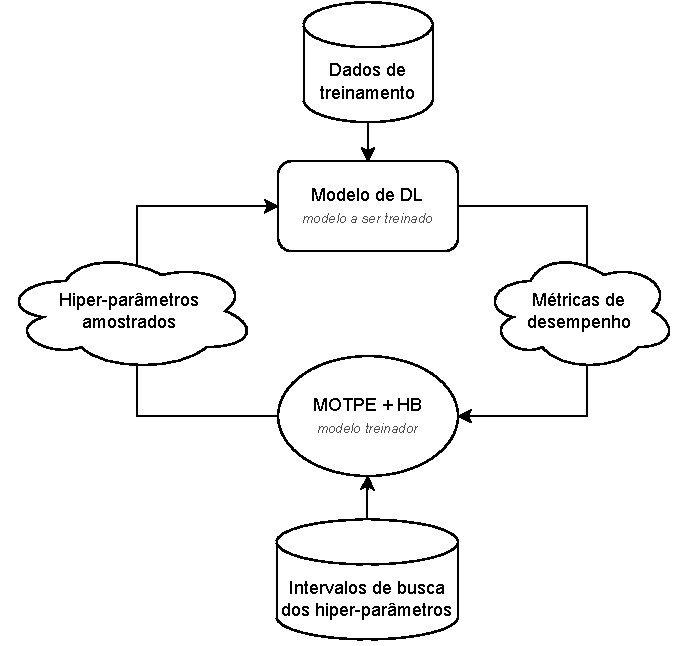
\includegraphics[width=0.85\textwidth]{figures/optuna.pdf}
%     \caption{Treino automático do modelo de DL por um modelo treinador, que faz a otimização dos hiperparâmetros iterativamente.}
%     \label{fig:optuna}
% \end{figure}



% \section{Resultados}
% \subsection{Métricas de Avaliação Quantitativa}
% \label{sec:metricas}

% \subsubsection{Acurácia}
% A acurácia representa o número de objetos classificados corretamente em relação ao número total de objetos. Sua expressão é mostrada na equação \eqref{eq:acuracia}.

% \begin{equation}
% \label{eq:acuracia}
% Acur\acute{a}cia = \frac{TP + TN}{TP + TN + FP + FN}
% \end{equation}%
% onde $TP$, $TN$, $FP$, e $FN$ são, respectivamente, a quantidade de Verdadeiro Positivo (\emph{True Positive}), Verdadeiro Negativo (\emph{True Negative}), Falso Positivo (\emph{False Positive}) e Falso Negativo (\emph{False Negative}).

% \subsubsection{Precisão e Recall}

% A acurácia nem sempre é uma métrica confiável para conjunto de dados desbalanceados, pois quanto maior a desproporção do número de objetos entre as classes, menor é o impacto das predições incorretas da classe em minoria no valor da acurácia, levando à uma avaliação superotimista do modelo. Para lidar com isso, usamos outras duas métricas: \emph{Precision} e \emph{Recall}, definidas nas equações \eqref{eq:precisao} e \eqref{eq:recall}, respectivamente.

% \begin{equation}
%   \label{eq:precisao}
%   Precision = \frac{TP}{TP + FP}
% \end{equation}

% \begin{equation}
%   \label{eq:recall}
%   Recall = \frac{TP}{TP + FN}
% \end{equation}

% As equações \eqref{eq:precisao} e \eqref{eq:recall} mostram que $Precision$ tem o valor máximo na ausência de Falso Positivo e $Recall$ tem o valor máximo na ausência de Falso Negativo. Ao adotarmos a classe em minoria como positiva, temos uma avaliação que reflete a capacidade do modelo na tarefa mais difícil -- a classificação correta de objetos na classe com menor representação no conjuto de treinamento.

% \subsubsection{F1-Score}
% Para sumarizar estas duas métricas, usamos uma outra, chamada $F_1$\emph{-score}, que é a média harmônica entre $Precision$ e $Recall$, como definida na equação \eqref{eq:f1}.

% \begin{equation}
%   \label{eq:f1}
%   F_1 = 2 \times \frac{Precision \times Recall}{Precision + Recall}
% \end{equation}





% \subsection{Avaliação do Modelo}
% \label{sec:avaliacao_melhor_modelo}

% \begin{figure}[!ht]
%   \centering
%   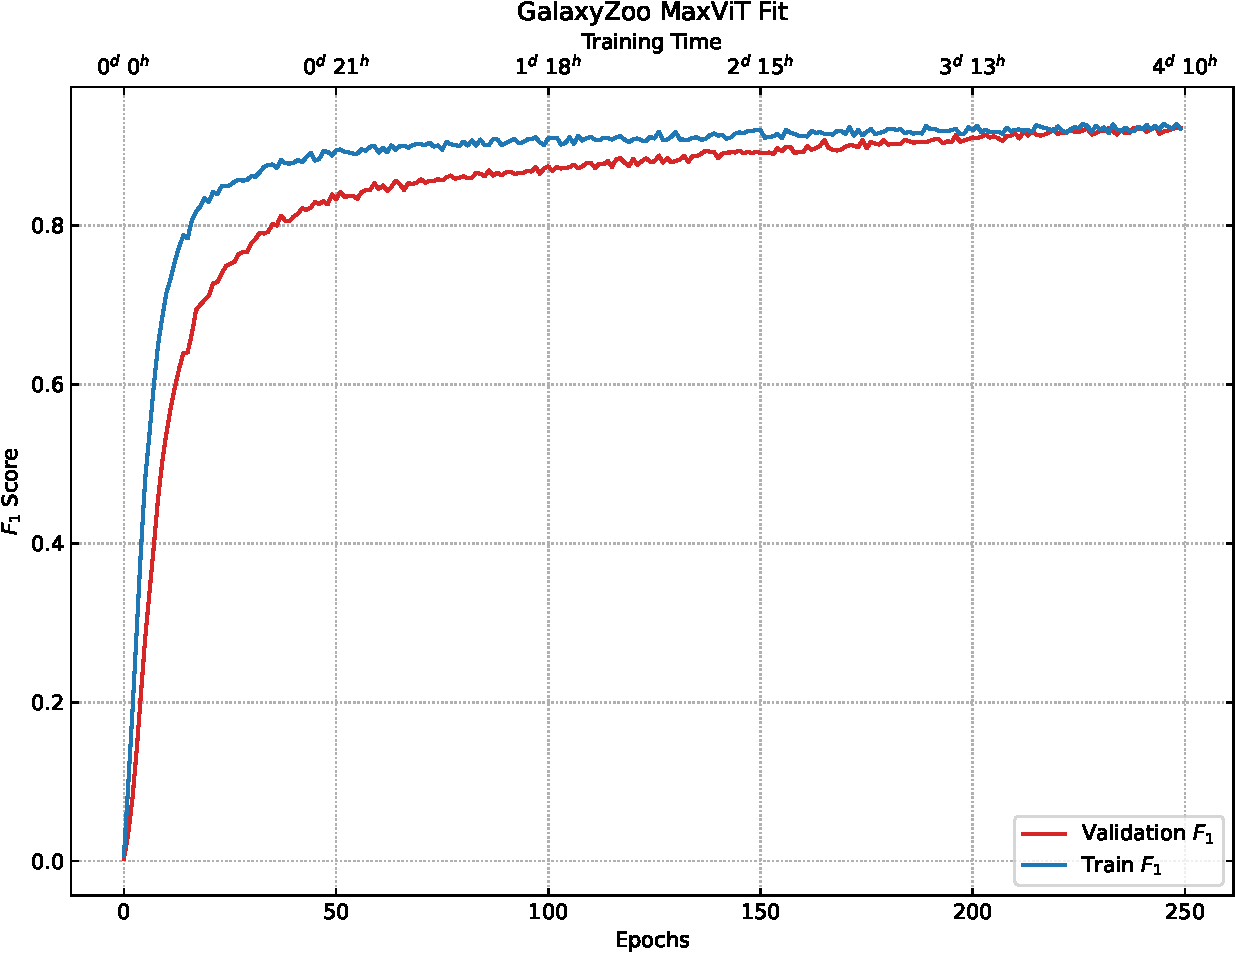
\includegraphics[width=\linewidth]{figures/train}
%   \caption{Evolução das métricas de avaliação do modelo durante o treino}
%   \label{fig:best_model_metrics}
% \end{figure}

% A curva de treinamento do modelo MaxViT (Fig. \ref{fig:best_model_metrics}) apresenta uma trajetória ascendente estável para o F1-Score de treinamento e validação, indicando que o modelo está aprendendo com os dados de treinamento de forma eficaz.

% A curva de treinamento converge em um valor alto de F1-Score (aproximadamente 0,8), sugerindo que o modelo está aprendendo os padrões relevantes nos dados de treinamento. Essa convergência indica que o modelo está encontrando um bom ajuste para os dados e não está apenas memorizando-os.

% A curva de F1-Score de validação acompanha de perto a curva de treinamento, com uma ligeira diferença entre elas. Essa diferença pode ser considerada um bom indicador da capacidade de generalização do modelo. Se a diferença fosse muito grande, isso poderia significar que o modelo está sobreajustando os dados de treinamento e não seria capaz de generalizar bem para novos dados.

% A curva de F1-Score de validação atinge um pico em torno da 150$^{a}$ época, seguido por uma ligeira queda. É importante verificar se essa queda é significativa ou se o modelo se estabiliza em um valor alto de F1-Score após a 150$^{a}$ época. Se a queda for significativa, isso pode indicar que o modelo está começando a sobreajustar os dados de treinamento e pode não generalizar bem para novos dados.


% A Fig. \ref{fig:best_model_metrics} mostra que o modelo apresenta um bom compromisso entre acerto de classificação e generalização no decorrer do treino, uma vez que as avaliações nos conjunto de treino e validação não apresentam divergência. 

% \begin{figure}[!ht]
%     \centering
%     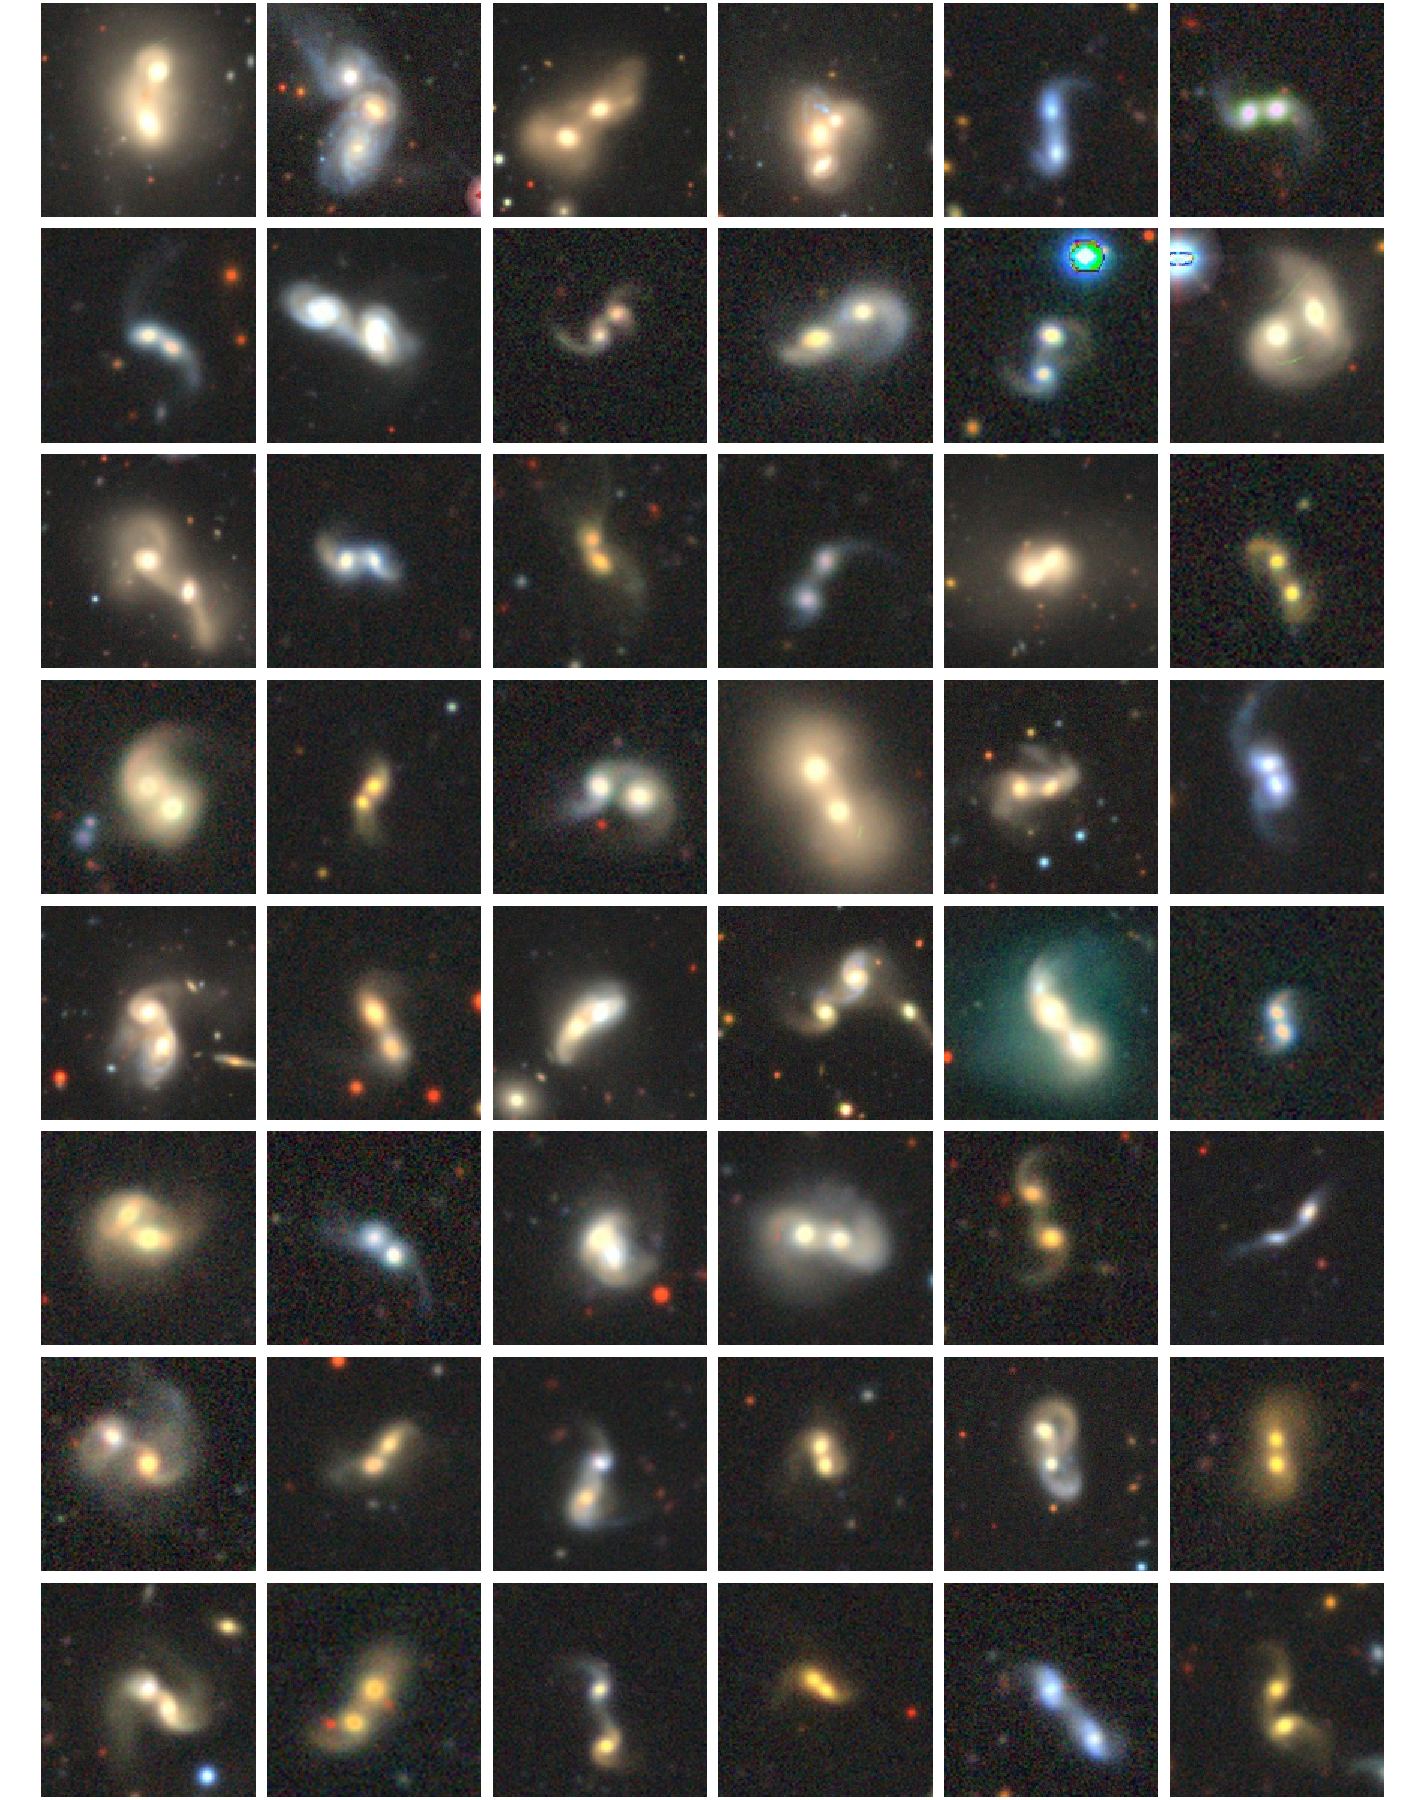
\includegraphics[width=\linewidth]{figures/desi_mergers.pdf}
%     \caption{Amostra de galáxias do Conjunto Cego (Seção \ref{sec:conjunto_cego}) contendo galáxias do hemisfério sul classificadas como \emph{merger}.}
%     \label{fig:blind_stamps_1}
% \end{figure}

% Já a Fig. \ref{fig:blind_stamps_1} possui uma amostra de galáxias mergers encontradas no Conjunto Cego (Seção \ref{sec:conjunto_cego}), mostrando a capacidade do modelo em aingir o objetivo de classificação em um conjunto de imagens diferente ao de treino.



% Com a classificação feita pelo modelo, o Conjunto Cego apresentou uma fração de mergers de aproximadamente 2.1\%. Contudo, após uma inspeção visual nos objetos classificados como mergers pelo modelo, foi constatada a existência significativa de falsos positivos. Desta forma, após a seleção visual dos objetos classificados automaticamente, a fração de objetos realmente mergers é foi de aproximadamente 0.95\%. A presença significativa de falsos positivos, já que a seleção dos hiperparâmetros foi feita de forma a maximizar a taxa de verdadeiros positivos, sem grandes penalizações para falsos positivos. O objetivo foi conseguir o maior número possível de galáxias mergers e depois fazer uma inspeção visual, pois esta tarefa manual pode ser rápidamente executada, pela peculiaridade visual das galáxias mergers.

% Os hiperparâmetros do modelo estão dispostos na Tabela \ref{tab:hiperparam_best}.

% \rowcolors{2}{white}{primaryColor!15!white}
% \begin{htable}{X|X}{Hiperparâmetros do melhor modelo}{\bf Hiperparâmetro & \bf Valor}{tab:hiperparam_best}
%     Learning Rate & 0.0001928999689128716\\
%     Weight Decay & 0.022222040734083764\\
%     Label Smoothing & 0.05193858928392769\\
%     Batch Size & 64\\
%     \hline
%     Dense Layer 1: Units & 1011\\
%     Dense Layer 1: Dropout & 0.2\\
%     Dense Layer 1: Batch Normalization & True\\
%     \hline
%     Dense Layer 2: Units & 586\\
%     Dense Layer 2: Dropout & 0.1\\
%     Dense Layer 2: Batch Normalization & True\\
%     \hline
%     Dense Layer 3: Units & 862\\
%     Dense Layer 3: Dropout & 0.2\\
%     Dense Layer 3: Batch Normalization & False\\
% \end{htable}


% \subsection{Interface de Consulta}

% O sistema implementado consta com uma interface de gráfica de busca que realiza toda operação de busca por similaridade na base de dados. A Fig. \ref{fig:ngc1011} mostra a consulta de galáxias similares à NGC 1011.

% \begin{figure}[!ht]
%   \centering
%   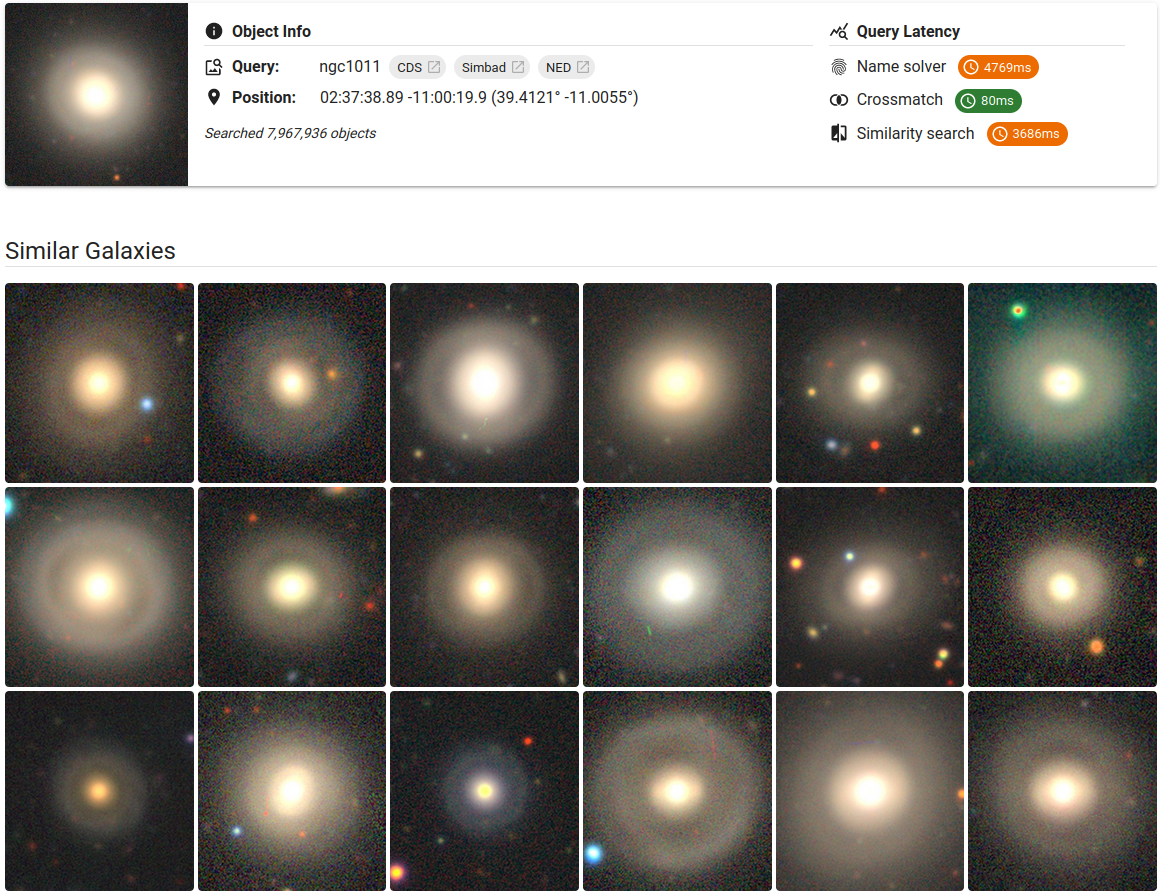
\includegraphics[width=\textwidth]{figures/ngc1011.png}
%   \caption{Interface gráfica do sistema mostrando as 18 galáxias mais parecida à galáxia buscada, NGC1011}
%   \label{fig:ngc1011}
% \end{figure}



% \section{Discussão e Conclusão}
% Nesta pesquisa, exploramos a eficácia do modelo MaxViT para a tarefa de classificação de imagens em múltiplas campanhas do Galaxy Zoo. Inicialmente, discutimos a arquitetura do MaxViT e suas vantagens em lidar com tarefas de visão computacional, destacando sua capacidade de capturar informações locais e globais por meio de atenç��o multi-eixo. Além disso, abordamos técnicas de treinamento e regularização utilizadas para melhorar o desempenho e a generalização do modelo.

% Ao avaliar quantitativamente o modelo, utilizamos métricas como precisão, recall e F1-Score para medir sua capacidade de classificação em conjuntos de dados desbalanceados. Os resultados mostraram uma convergência estável das métricas de avaliação durante o treinamento, indicando que o modelo está aprendendo de forma eficaz e sendo capaz de generalizar para dados não vistos.

% Uma interface web para consulta de imagens por similaridade oferece uma plataforma intuitiva e acessível para os usuários explorarem grandes conjuntos de dados visuais de maneira eficiente e eficaz. Ao permitir que os usuários busquem por uma imagem de consulta, essa interface utiliza algoritmos de busca por similaridade visual, como o HNSW, combinados com embeddings de modelos como o MaxViT, para recuperar imagens semelhantes a partir de um banco de dados vasto. Isso proporciona uma experiência de busca visualmente rica, onde os usuários podem descobrir imagens relacionadas com rapidez e precisão, facilitando tarefas como encontrar inspiração criativa, identificar objetos específicos ou explorar conceitos visuais.

% Uma das principais vantagens de uma interface web para consulta de imagens por similaridade é sua acessibilidade universal. Ao fornecer uma plataforma baseada na web, os usuários podem acessar a ferramenta a partir de qualquer dispositivo conectado à Internet, incluindo computadores desktop, laptops, tablets e smartphones. Isso torna a busca por imagens por similaridade uma tarefa conveniente e flexível, permitindo que os usuários explorem conteúdo visual de forma intuitiva em qualquer lugar e a qualquer momento.

% Além disso, uma interface web para consulta de imagens por similaridade oferece uma experiência interativa e envolvente, enriquecida por recursos como visualização de resultados, filtragem por categoria e personalização de preferências de busca. Essa abordagem centrada no usuário torna a busca por imagens uma experiência altamente personalizada e adaptável, atendendo às necessidades individuais e preferências dos usuários. Ao combinar a potência dos algoritmos de busca por similaridade visual com a facilidade de uso de uma interface web, essa ferramenta se destaca como uma solução poderosa para explorar e descobrir conteúdo visual de forma eficiente e intuitiva.

% Em conclusão, os resultados obtidos até o momento são encorajadores, demonstrando o potencial do modelo MaxViT para a classificação de imagens em conjuntos de dados desbalanceados. No entanto, são necessárias análises adicionais e ajustes para garantir a eficácia e a robustez do modelo em diferentes cenários de aplicação. Futuros trabalhos podem se concentrar em investigar ainda mais as causas da queda no desempenho e explorar estratégias adicionais para melhorar a capacidade de generalização do modelo.

% A análise do comportamento do modelo durante o treinamento é fundamental para entender como ele aprende ao longo do tempo. Os gráficos de acurácia, custo, recall e F1-Score ao longo das épocas de treinamento  (Fig. \ref{fig:best_model_metrics}) mostram que o modelo escolhido não sofre de \emph{overfitting}, pois não há divergência entre as métricas de treino e validação. Isso indica que o modelo está generalizando bem para dados não vistos, o que é essencial para sua aplicação em um conjunto de galáxias diferentes.

% Uma das evidências mais críticas do desempenho do modelo é sua capacidade de classificar galáxias mergers em um conjunto de dados desconhecido. A amostra de galáxias mergers apresentada no Conjunto Cego (Seção \ref{sec:conjunto_cego}) é promissora, demonstrando que o modelo é capaz de identificar adequadamente esse tipo de galáxia.

% Essa capacidade de generalização é fundamental, uma vez que a tarefa de classificar galáxias mergers em observações reais exige que o modelo possa identificar esses objetos em um contexto totalmente diferente do conjunto de treinamento.

% Desta maneira, este estudo demonstra que é possível treinar um modelo de aprendizado profundo para a tarefa desafiadora de classificar galáxias mergers com base em imagens. A otimização de hiperparâmetros desempenha um papel crucial na obtenção de um modelo com bom desempenho.

% No entanto, é importante observar algumas limitações deste estudo. Primeiramente, o modelo foi treinado e avaliado em um conjunto de dados limitado, que o impede de ser uma representação fiel do universo. Além disso, há algumas restrições criadas durante a concepção do modelo, como a escolha da arquitetura da CNN e dos hiperparâmetros a serem otimizados. Portanto, a generalização do modelo para outras tarefas ou conjuntos de dados requer análises adicionais.

% Além disso, a capacidade de identificar galáxias mergers depende em parte da qualidade e resolução das imagens de entrada. Em observações reais, a qualidade das imagens pode variar significativamente, o que pode afetar o desempenho do modelo.

% Para futuras melhorias, é possível considerar a expansão do conjunto de treinamento com uma variedade maior de imagens e a exploração de arquiteturas de CNN mais complexas. Além disso, a implementação de técnicas de aumento de dados pode aumentar a capacidade do modelo de generalizar para diferentes condições de observação.




% A Figura \ref{fig:sky-distrib} mostra a distribuição de cada objeto no céu. Nela é possível ver que há pouca intersecção dos objetos catalogados com objetos do S-PLUS, pois os catálogos obtidos são baseados em levantamentos do hemisfério norte. Sendo assim, serão testadas técnicas de transferência de conhecimento para 


% \begin{figure}[!ht]
%   \centering
%   \includegraphics[width=\textwidth]{figures/sky_distrib.pdf}
%   \caption{Distribuição no céu dos conjuntos S-PLUS Blind, GZ-1 \citep{gz1}, GZ-Decals \citep{gzdecals} e Darg \citep{darg-a, darg-b}}
%   \label{fig:sky-distrib}
% \end{figure}


% \bibliographystyle{plainnat}
% \bibliography{refs}
\printbibliography


\horizonBackCover
\end{document}
